\selectlanguage{english}
\chapter{Building Efficient Domain-Specific Memory Profilers}
\label{chp:dsl-memory}
\markboth{Building Efficient Domain-Specific Memory Profilers}{Chapter6}

\coolphrase{This is something here}{Fight Club}

%#Context  
%Domain-specific abstractions are increasingly used in industry to ease the development of applications. These abstractions take various forms, (e.g., domain-specific languages (DSL), macros, component models). Workbenches exist to define tooling over such abstractions. For example, DSL workbenches support the development of editors and code generators. 
% #Problem 
%However, profiling applications which use these abstractions requires significant development efforts to keep the traceability links between these abstractions and the runtime data-structures. This effort must be balanced with the limited audience of these abstractions. 
%Sate of the art profilers are able to represent such abstractions through generic query evaluation, but they suffer from bad performance issue. 

%#Contribution
%In this paper, we propose an approach to ease the development of efficient memory analysis tools to be used during the production stage.
%Our approach provides a DSL to express the mapping between abstractions and runtime data structure.
%At runtime, the generated  memory analysis tools leverage the object graph traversal mechanism to efficiently collect the specific memory data required.
%#Evaluation
%To evaluate our approach, we compare memory analysis tools produced with our DSL against: i) hand written optimized solutions, and ii) solutions based on existing tools which offer lower performance.
%The results show that our approach offers performance gain compared to previous solutions, and simplify the definition of memory analysis tools.

\lstset{frame=t,
  aboveskip=1mm,
  belowskip=1mm,
  showstringspaces=false,
  columns=flexible,
  basicstyle=\color{black}\scriptsize,
  numbers=none,
  numberstyle=\color{gray}\scriptsize,
  keywordstyle=\color{black}\scriptsize\bfseries,
  commentstyle=\color{dkgreen}\scriptsize,
  stringstyle=\color{purple}\scriptsize,
  identifierstyle=\color{dkgray}\scriptsize,
  breaklines=true,
  breakatwhitespace=true,
  tabsize=4,
  captionpos=b,
}

\lstdefinelanguage{AlgLang}
{
literate={aaa}{bbb}3,
morekeywords={input, foreach, action, if, return, routine, values},
morekeywords={instances_for, have_id},
sensitive=true,
frame=tblr,
morecomment=[l]{//},
morecomment=[s]{/*}{*/},
morestring=[b]",
}

\lstdefinelanguage{DSL}
{
literate={aaa}{bbb}3,
morekeywords={data, set_type, void, int, bool, Objects, THIS, is, ENTITY},
morekeywords={instances_for, have_names},
sensitive=true,
morecomment=[l]{//},
morecomment=[s]{/*}{*/},
morestring=[b]",
}

\lstdefinelanguage{OCL}
{
literate={aaa}{bbb}3,
morekeywords={context,inv,and,or,self},
sensitive=true,
frame=tblr,
morecomment=[l]{//},
morecomment=[s]{/*}{*/},
morestring=[b]",
}

\lstdefinelanguage{DSL2}
{
literate={aaa}{bbb}3,
frame=tblr,
%numbersep=2pt,
numbers=left,
numberstyle=\color{black}\scriptsize,
morekeywords={void, int, bool, in, is, or, and},
morekeywords={membership, initialValues, updates, structure, initialObjects, create, using, constructor, foreach},
sensitive=true,
morecomment=[l]{//},
morecomment=[s]{/*}{*/},
morestring=[b]",
ndkeywords={false, true, this, referrer, threads, this_structure},
ndkeywordstyle=\color{blue}\bfseries
}

\lstdefinelanguage{OQL}
{
literate={aaa}{bbb}3,
morekeywords={SELECT, FROM, WHERE, UNION, AS, DISTINCT, ALL, GROUP, BY},
sensitive=true,
frame=tblr,
morecomment=[l]{//},
morecomment=[s]{/*}{*/},
morestring=[b]",
}

\lstdefinelanguage{CYPHER}
{
literate={aaa}{bbb}3,
morekeywords={MATCH, RETURN, WITH, sum},
sensitive=true,
frame=tblr,
morecomment=[l]{//},
morecomment=[s]{/*}{*/},
morestring=[b]",
}


%\section{Introduction}\label{sec:introduction}
%Garbage collection-based memory management is a wide\-spread approach nowadays since
%it improves software quality and eases the development process.
%Nonetheless, memory-related issues are still relevant in languages/runtimes with
%garbage collectors because developers tend to fail during memory manipulation.
%In particular, it is known that memory leaks and unnecessary allocations are the sources
%of both functional and non-functional software misbehavior~\cite{cbse/14/attouchi/monitoring, Vera:2004:FAF:973097.973099}.

%Dealing with these issues have been a concern for both the industry and the academy
%for a while; therefore, there are several approaches to reduce the risk of memory-related
%errors.
%In the industry, practitioners use memory profilers (e.g. YourKit, Eclipse Memory
%Analyzer Tool and Plumbr) to deal with the problem.
%These tools support many sort of built-in analysis which are fairly efficient because
%they are based on industrial standards such as JVMTI.
%Some of them also provide mechanisms to specify user-defined analysis through a query 
%language such as OQL~\cite{OQL-visualvm}.
%Although useful, the usage of user-defined analysis requires in most cases the 
%generation of a costly heap dump which makes the associated queries unsuitable for
%at runtime execution in a production environment.
%Hence, it is not possible to use these tools to feed neither self-adaptive nor self-healing
%systems.

%In the academy, different approaches tackle memory issues~\cite{Xu:2015:MPP:2729552.2729565, Nguyen:2007:DEM:1296907.1296912, Bond:2008:TML:1449764.1449774, Jung:2014:AML:2568225.2568311}.
%Many of these solutions are either efficiently implemented as hard-coded modifications to the
%garbage collector or built on top of industrial standards as JVMTI.
%The advantage of these mechanisms is a reduction on the overhead of such analysis.
%However, they have two limitations: i) they target a single memory issue and ii) it is hard to
%introduce them in the industry.
%In general, implementing a highly efficient analysis requires knowledge of low-level APIs or
%garbage collection mechanisms which are not commonly in the curriculum of most managed runtime
%environment (MRE) users.

%It seems clear to us that there is a gap in existent solutions to analyze the heap.
%Either they are fairly {\em generic/easy to use} but offer poor performance or they offer good performance but are hard to customize/create. 
%We claim that a {\em simple to use} and efficient mechanism to perform memory analysis is
%a feature required in many areas of software development for MREs (e.g. to build self-adaptive systems, to
%reduce development complexity, to decrease the number of errors).  

%In this paper, we propose a framework to analyze the status of the memory heap and collect information about it.
%The main component of the framework is a domain-specific language (DSL) that allows us to specify
%how to explore and collect the desired information.
%The concepts of this language are highly coupled to the way the heap is traversed.
%A program in this language is compiled into a backing technology that support, in an efficient way, the iteration over all objects and 

%New software abstractions are created for good reasons, such as  having specific point of views on a particular system, simplifying software development, reducing errors, removing redundant tasks and improving productivity. 
%There is currently a trend in \glslink{SE}{SE} towards the creation of new languages and tools to support specific software developments~\cite{whittle2014state, van2000domain,hutchinson2011empirical}. 
%The design of such new languages and platforms are done for good reasons, such as  having specific point of views on a particular system, simplifying software development, reducing errors, removing redundant tasks and improving productivity. 
%This trend has led to the development of new research topics such as .
The \gls{SLE} community aims at reducing the effort required in engineering new languages and their corresponding development tools, thus improving the efficiency of both people in charge of designing new languages and their users~\cite{sle}. 
However, as far as we know, they do not take into account profiling tools, which are essentials for software maintenance and optimization.
Indeed, although specific tools are needed to monitor running systems in order to detect defects or abnormal behaviors~\cite{duesterwald2000software, Jovic:2011:CMY:2076021.2048081},
little support exists to ease their creation.

%Many of the newly designed languages and runtime platform are built on top of existing object oriented languages runtime such as the Java Virtual Machine (JVM). 
%Therefore people in charge of optimizing, debugging and maintaining software applications can use the existing debugger and profilers of these platforms. 
%However, there is a paradigm mismatch between the classical profilers used in object-oriented systems and the newly designed platforms and languages. 
%Indeed, the concepts introduced in these new languages may not exhibit a straightforward mapping to the underlying object-oriented system. For example, in the Spring framework~\cite{laddad2009aspectj}, some annotations like $@Aspect$ generate dynamic proxies on the fly. Existing profilers will present these proxies as normal objects, thus revealing a mismatch between the profiler and developer view. 

In this chapter, we focus on the problem of easing the creation of memory profilers for domain-specific software abstractions that are designed to be executed on top of MRTEs. 
We first propose a metalanguage to specific what data about the memory use is of interest in a domain (see Section~\ref{sec:approach}).
A profiler is then generated to collect the data and present it in terms of concepts of that language. 
In addition, we present a tooled DSL based on such a metalanguage, which generates profilers for the JVM (see Section~\ref{sec:implementation}).
%to match the language concepts and provide useful information to the end user.
An important point of our approach is the low overhead induced by these profilers; this makes them usable in production environments (see Sections~\ref{sec:expressiveness} and~\ref{sec:dsl-evaluation}).
%Indeed, generating a specific profiler from an abstract definition of the role of this profiler enable us to produce very specific profiler which only monitor the relevant information.

The contributions of this chapter are as follows:
\begin{itemize}
\item A metalanguage to describe what information a profiler must collect.
In addition, programs in this metalanguage also defines how to collect the information.
Although knowledge of the underline execution model is required, the procedure to obtain data is mostly defined without using low-level details.  

\item A concrete implementation of this metalanguage that target the JVM.
In particular, by using the \glslink{JVMTI}{JVMTI}, we are able to generate memory profilers with low overhead.
Concrete profilers already generated are portable to any implementation of the JVM that supports JVMTI.

\item A discussion of the metalanguage's expressiveness, and an evaluation of the performance overhead induced by three profilers in real-world use cases.
\end{itemize}

%The rest of this chapter is organized as follows
%A description of the DSL and its tooling support are presented in sections and .
%In section we discuss the expressiveness of the language.
% presents an evaluation of the performance achieved by the custom profilers.
%Related works are discussed in section~\ref{sec:relatedwork}.
%Finally, section~\ref{sec:conclusions} gives the conclusions and presents future works.

%\section{Background and motivating example}\label{sec:background}

%\subsection{Motivating example\label{sec:motivatingexample}}

%In this section we present a motivating example for the use of an optimistic adaptive monitoring process in the context of a real-time crisis management system in a fire department. 
During a dangerous event, many firefighters are present and need to collaborate to achieve common goals.
%In a situation where many firefighters are present and need to collaborate to handle a dangerous event, 
Firefighters have to coordinate among themselves and commanding officers need to have an accurate real-time view of the system.

The Daum project\footnote{\url{https://github.com/daumproject}} provides a software application that supports firefighters in these situations.
The application runs on devices with limited computational resources because it must be mobile and taken on-site.
%As the software have to be mobile to take it on site, it is running on devices with limited computation resources.
It provides numerous services for firefighters depending on their role in the crisis.
In this chapter, we focus on the two following roles:
\begin{itemize}
\leftskip -.2in
 \item A collaborative functionality that allows commanding officers to follow and edit tactical operations. The firefighters' equipment include communicating sensors that report on their current conditions.
 \item A drone control system which automatically launches a drone equipped with sensors and a camera to provide a different point-of-view on the current situation.
\end{itemize}

%\todo{I don't get this for example. It is not relate to the previous sentence.}For example, one service is related to firefighter information monitoring to know the location, activity and health status of each firefighter involved on the crisis but also to get some information on their environment (e.g. temperature, toxic gas). Another service is in charge of the management of victims. They must be redirected according to their needs.

As is common in many software applications, the firefighter application may have a potentially infinite number of configurations. These configurations depend on the number of firefighters involved, the type of crisis, the available devices and equipment, among other parameters. 
Thus, it is generally not possible to test all configurations to guarantee that the software will always function properly. 
Consequently, instead of testing all configurations, there is a need to monitor the software's execution to detect faulty behaviours and prevent system crashes. 
However, fine-grained monitoring of the application can have excessive overhead that makes it unsuitable with the application and the devices used in our example.
Thus, there is a need for an accurate monitoring system that can find faulty components while reducing overhead.

The Daum project has implemented the firefighter application using a Component Based Software Architecture.  The application makes extensive use of the Kevoree\footnote{\url{http://www.kevoree.org}\label{note:kevoree}} component model and runtime presented in chapter \ref{chap:abstractions_and_resource_management}.

% Using our adaptive monitoring solution, we are able to reduce the overhead of the monitoring process keeping enough well response time to find faulty behaviors.



\subsection{Kevoree}
Kevoree is an open-source dynamic component platform, which relies on Models@run.time~\cite{BlairBF09} to properly support the dynamic adaptation of distributed systems.
Our use case application and the implementation of the Scapegoat framework make extensive use of the Kevoree framework.
The following subsections detail the background on component-based software architecture, introduce the Models@run.time paradigm and give an overview of the Kevoree platform.

\subsubsection{Component-based software architecture}

Software architecture aims at reducing complexity through abstraction and separation of concerns by providing a common understanding of component, connector and configuration~\cite{xadl,Medvidovic:2000,VanOmmering-et-al-00}.
One of the benefits is that it facilitates the management of dynamic architectures, which becomes a primary concern in the Future Internet and Cyber-Physical Systems~\cite{DBLP:journals/ase/NittoGMPP08, Johnson:2015:CSM:2735960.2735979}.
Such systems demand techniques that let software react to changes by self-organizing its structure and self-adapting its behavior~\cite{PanzicaLaManna:2012:LDU:2304736.2304764, Johnson:2015:CSM:2735960.2735979, Zhang:2009:MVD:1509239.1509262}.
Many works~\cite{cbse-conference} have shown the benefits of using component-based approaches in such open-world environments~\cite{baresi2006toward, Caporuscio:2010:AIA:1985522.1985547, Perez-Palacin:2010:PAO:1712605.1712614}.

To satisfy the needs for adaptation, several component models provide solutions to dynamically reconfigure a software architecture through, for example, the deployment of new modules, the instantiation of new services, and the creation of new bindings between components~\cite{Porter:2014:RMC:2602458.2602471, Zheng:2014:RCC:2679601.2680405, Irmert:2008:RAS:1370018.1370036, Ghezzi:2010:QDD:2163764.2163774}. 
In practice, component-based (and/or service-based) platforms like Fractal~\cite{bruneton06}, OpenCOM~\cite{BlairCULJ04}, OSGi~\cite{OSGI:r5} or SCA~\cite{SEINTURIER:2011:INRIA-00567442:1} provide platform mechanisms to support dynamic architectures.

%As a result, component-based platforms offer a challenging playground for building adaptive monitoring framework as they raise a new challenge in easing the open-world paradigm and they can be an element of the solution. 

%In this context, traditional software development, based on the closed-world assumption that the  boundary between system and environment is known and unchanging does not work.


\subsubsection{Models@run.time}
Built on top of dynamic component frameworks, Models@run.time denote model-driven approaches that aim at taming the complexity of dynamic adaptation.
It basically pushes the idea of reflection~\cite{morin09a} one step further by considering the reflection-layer as a real model: ``something simpler, safer or cheaper than reality to avoid the complexity, danger and irreversibility of reality''.
In practice, component-based and service-based platforms offer reflection APIs that allow instrospecting the application (e.g., which components and bindings are currently in place in the system) and dynamic adaptation (e.g., changing the current components and bindings).
While some of these platforms offer rollback mechanisms to recover after an erroneous adaptation~\cite{leger2010reliable}, the purpose of Models@run.time is to prevent the system from actually enacting an erroneous adaptation. 
In other words, the ``model at runtime'' is a reflection model that can be decoupled from the application (for reasoning, validation, and simulation purposes) and then automatically resynchronized.
This model can not only manage the application's structural information (i.e., the architecture), but can also be populated with behavioural information from the specification or the runtime monitoring data.


\subsubsection{The Kevoree framework\label{sec:kevoree}}	
% Se proteger un peu plus sur Kevoree pour big node / placer plus de ref / comparaison ?
%Language

%\todo{THIS SECTION IS VERY UNCLEAR!!!}

Kevoree provides multiple concepts that are used to create a distributed application that allows dynamic adaptation. The \emph{Node} concept is used to model the infrastructure topology and the \emph{Group} concept is used to model the semantics of inter-node communication, particularly when synchronizing the reflection model among nodes. 
Kevoree includes a \emph{Channel} concept to allow for different communication semantics between remote \emph{Components} deployed on heterogeneous nodes. 
All Kevoree concepts (\textit{Component}, \textit{Channel}, \textit{Node}, \textit{Group}) obey the object type design pattern~\cite{johnson_type_1997} in order to separate deployment artifacts from running artifacts.  

%Platforms
Kevoree supports multiple execution platforms (e.g.,~Java, Android, MiniCloud, FreeBSD, Arduino). For each target platform it provides a specific runtime container. 
%Tools
Moreover, Kevoree comes with a set of tools for building dynamic applications (a graphical editor to visualize and edit configurations, a textual language to express reconfigurations, several checkers to valid configurations). 

%The remainder of this section describes the main concepts of the Kevoree component model that are useful to understand the scapegoat approach.
%\todo{One sentence to explicit how Kevoree and Model@Runtime help the development of our approach}

As a result, Kevoree provides a promising environment by facilitating the implementation of dynamically reconfigurable applications in the context of an open-world environment.
Because our goal is to design and implement an adaptive monitoring system, the introspection and the dynamic reconfiguration facilities offered by Kevoree suit the needs of the ScapeGoat framework.
%As a result, component-based platforms offer a challenging playground for building adaptive monitoring framework as they raise a new challenge in easing the open-world paradigm and they can be an element of the solution. 



%\subsection{Dynamic Adaptation with Kevoree}
%Kevoree aims at providing advanced adaptation capabilities to different types of nodes:
%\begin{itemize}
%\setlength{\itemsep}{0pt}
%\setlength{\parskip}{0pt}
%\setlength{\parsep}{0pt}
%\item 
%\noindent{\bf Level 1: Parametric adaptation.} Dynamic update of parameter values, e.g. change of sampling rate in a component that wraps a physical sensor (adaptation of instance properties).

%\item 
%\noindent{\bf Level 2: Architectural adaptation.} Dynamic addition or removal of bindings or components, e.g. replication of software components and channels on different nodes to perform load balancing (adaptation of instances graph).

%\item 
%\noindent{\bf Level 3: Dynamic provisioning of types.} Hot deployment of component types that were not foreseen before the initial deployment of the system. 
%This allows for system evolution by enabling parametric and architectural reconfigurations, including management of instances for types that are added and managed dynamically (adaptation of types).

%%\item 
%%\noindent{\bf Level 4: Adaptation for remote management.} Nodes supporting level~4 adaptation participate in a remote management layer, which supervises less powerful nodes. 
%%This layer monitors remote nodes by requesting their current Kevoree model;
%%the layer triggers dynamic adaptation of nodes by sending precomputed reconfiguration scripts to them. 
%%This remote adaptation process supports seamless management of less powerful nodes by a more powerful one, which has enough resources to build and evaluate new and appropriate  configurations.
%\end{itemize}

%The adaptation engine relies on a model comparison between two Kevoree models to compute a  script for a safe system reconfiguration; execution of this script brings the system from its current configuration to the new selected configuration~\cite{morin09a}. 
%Model comparison yields  a delta-model defining changes (using CRUD operations) that should be applied on the source model to obtain the target model. 
%Planification algorithms~\cite{daubert} use this delta-model as input in order to defined an efficient schedule of the adaptation steps. 
%The delta-model is finally compiled into a Kevoree script. 
%The Kevoree Script language (KevScript for short) is a core language for describing reconfiguration.
%KevScript  is comparable to FScript for Fractal Component Model~\cite{DBLP:journals/adt/DavidLLC09}. 
%Execution of a KevScript directly adapts a Kevoree system, without the need for  a full Kevoree model definition. 
%Such adaptation scripts are written by designers, or they can be generated  by automated processes ({\em e.g.} within a  control loop managing the Kevoree system).

%\hl{(Johann) What is the point of having so much detail about the Kevoree adaptation framework for this paper? It's not clear to me or we should have a last paragraph explaining a bit in what this is usefull for the rest of the paper.}


%\section{Motivating examples}\label{sec:motivation}
%For the motivating example talk about the case of online memory consumption monitoring.
%Explain how it is useful to perform the monitoring stage of the MAPE Loop.
%Explain the particular case of Component-Based Software Systems built on top of Java (e.g. OSGi, Kevoree)
Online application performance monitoring is an important concern to detect misbehavior, failures or even potential attacks.
%Self-adaptive and autonomic systems~\cite{kephart2003vision} are systems capable of dynamically adapting their behavior in reponse to changes in their execution environment (failure, performance degradation and so on).
%Self-adaptive systems are generally following a standard architecture called the MAPE-K loop~\cite{Huebscher:2008:SAC:1380584.1380585} which stand for
%Monitoring, Analysis, Planning and Execution.
%Monitoring is the step where the control loop collects meaningful information to drive the system adaptations.
%A self-adaptive system must thus collect data regarding computational resource consumption in order to be resource-aware~\cite{Maheo:2004:MSD:1018420.1019675, Simao:2012:VEJ:2310096.2310158, Guidec:2003:JMP:1899290.1899304}.
At the same time, online memory usage monitoring and analysis is a complex problem when the application development has leveraged specific abstractions. 
This section discusses three examples in which developers use specific abstractions provided by a framework or by themselves. 
For each of these examples, we illustrate the mismatch between the concepts used by developers and the concepts manipulated by the state of the art profiling tools. 

Our first example refers to the use of active annotations in the Xtend~\cite{bettini2013implementing} language.
Active annotations allow developers to participate in the translation process of Xtend source code to Java code via library.
This is particularly useful when Java requires to write a lot of boilerplate manually. 
For instance, many of the good old design patterns fall into this category. 
An active annotation is an annotation declared either in Java or Xtend, which is itself annotated with Active. 
\textit{@Active} takes a type literal as a parameter pointing to the processor. 
It can be seen as a subset of the macro mechanism that exists in Scala or Smalltalk~\cite{burmako2013scala}. 
Such mechanism is often used directly by developers to introduce their own abstraction or defining their own internal DSL. 
For example, in the K3-AL\footnote{Available at https://github.com/diverse-project/k3/wiki} project, we use active annotations to create an open-class mechanism in Java~\cite{Clifton:2000:MMO:353171.353181}. 
As a result, the annotation processor change the program structure to implement this feature. 
It adds some methods indirection (to $AASpect$), create new set of objects that represents the state of one conceptual object ($AASpectProperty$), use the Xtend extension method feature, etc\dots 
Figure~\ref{fig:famous} shows the result of this translation process. 
The left part illustrates the code written by the developer, the middle part shows the developer view (the code that can be written to use the open-class mechanism), the right part describes the runtime view. 
 
The current issue is the lack of traceability in the translation process. 
As a result, the abstraction used by the profiler does not match the abstractions used by the developer. 
Adapting profiling tools for these abstractions still requires significant development efforts that must be balanced with the limited audience of these abstractions.

\begin{figure*}
\centering
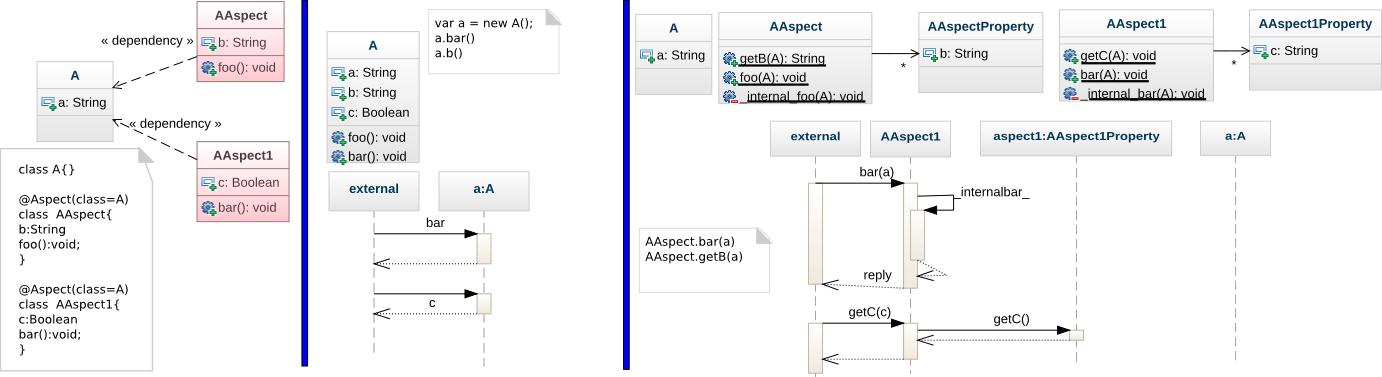
\includegraphics[width=0.9\linewidth]{chapter6/fig/famous}
\caption{Translation process used for building developer abstraction using annotations}
\label{fig:famous}
\end{figure*}

An other example is the OSGi framework. 
In OSGi, developers and users deploy many bundles on top of a single JVM.
It is therefore very complex to decide which bundle should be accounted for the consumption of a particular object because the heap is shared by all the bundles.
A solution to this problem is to account an object $O$ to a bundle if the object $O$ was loaded using the classloader $C$ associated with such a bundle: you can find a path from $C$ to $O$ in the graph of live objects.
This particular solution can be implemented because the mapping between bundle and Java abstractions is known. 
Hence, we can hard-code this mapping in a specific profiler written by hand or we can modify the garbage collector.
Nonetheless, different component-models implementations may map components to different Java abstractions; therefore, the previous solution does not work for all of them.
Thus developers must design and implement specific profilers from scratch for each framework and specific abstractions they are using. 
This is a very error prone, hard to debug and time consuming task. 

Finally, the Spring Framework provides a comprehensive programming and configuration model for modern Java-based enterprise applications - on any kind of deployment platform. 
A key element of Spring is its infrastructural support at the application level.
Spring focuses on all the repetitive manual tasks a developer has to handle when developing enterprise applications so that teams can focus on the business logic, without unnecessary ties to specific deployment environments. 
To take care of all these repetitive tasks, Spring provides Dependency Injection, Aspect-Oriented Programming including Spring's declarative transaction management, RESTful web service framework, support for JDBC, JPA, JMS, \dots. 
For all these features, Spring provides abstractions through Java annotations for developers, injects at runtime dynamic proxies to handle these repetitive tasks and adapts the wiring of objects. 
As a result, it exists a mismatch between the running set of objects and the application design. 
This mismatch makes the application profiling difficult and error prone. 


\section{Understanding the domain} \label{sec:domain-overview}

The purpose of memory profilers is capturing information regarding how applications use memory.
To write profilers, a clear understanding about their nature is required.
Informally, the term \textit{memory profiling} refers to any kind of \textbf{process to collect} some \textbf{data about memory usage}.
In an object-oriented runtime environment, such data may be as simple as the number of objects of a specific class, but it may also be as complex as the list of possible memory leak's sources.
Some other examples include computing the number of objects reachable from a specific class object; finding out if there is an instance of class $A$ which is referencing an object of class $B$; and computing, for each \textit{String}, its length and the number of objects that make direct reference to the \textit{string}.
The data collected by a profiler may have an arbitrary complexity; it may be a simple natural number, a boolean value, a list of values, or a composed value.
For instance, an integer value is required to describe one of the aforementioned examples, the number of objects reachable from a specific class object.
In the same way, a pair $\langle l,r \rangle$, where both $l$ and $r$ are integers, is required to store the result of determining for a \textit{string}, its length and the number of objects referencing it.
%The data collected by a profiler may have an arbitrary complexity

%The rest of this section introduces the vocabulary we use in the domain of memory profilers.

Formally, we use a set of concepts to properly define our understanding of the term profiler, and how we address their construction in this chapter.
The following concepts are used int the rest of the chapter:

\begin{description}
\item[Object] is an atomic entity that consumes memory to store the value of its attributes.
When we say \textit{object} we mean as in \gls{OOP}.
The operations that we can perform on these objects are nevertheless restricted to accessing attributes, obtaining the amount of memory used to represent an object, and accessing meta-data such as the class name.
Reusing the concept is ``natural'' since we are targeting MRTEs, which often support the object-oriented paradigm.

\item[Memory Heap] As mentioned, this is the region of memory used to store dynamically allocated \textit{objects} that are connected through references -- forming a directed-acyclic graph.
It is also the universe $\mathbb{U}$ of objects.

\item[Structure] is a subset of \textit{objects} in the \textit{memory heap}.
The objects in a structure don't need to be directly related by references; instead, they can be arbitrarily composed.
For instance, the smallest non-empty \textit{structure} we can consider, is a structure containing a single object.
Only one property is required in properly formed structures;  $S_1 \bigcap S_2 = \emptyset$ for any pair of structures $S_1$ and $S_2$, which means that they are disjoint sets.

\item[Memory Profile] is a value that can be computed using information from the \textit{objects} (and their references) included in a \textit{structure}.
An example of useful value is the total size of a structure, which can be easily calculated using the function $\textit{total\_size}\left(S\right) = \sum_{o \in S} {sizeof(o)}$.
A common pattern of use is to identify many \textit{structures} in the heap, and then to compute a value -- not necessarily the same -- for each structure.

\item[Memory Profiling] consists in identifying \textit{structures}, and computing some values associated to these structures. 

\item[Structure types] provide a mean to identify several structures using a single description.
In other words, since the heap can be partitioned in many structures, it is hard to manually enumerate them.
We need a procedural way to describe what are the structures we are considering (i.e., their membership functions), and what data we want to compute on each one of them; \textit{structure types} provide such facilities.

%Structure types parametrizado 
In particular, they provide (i) functions to evaluate whether an object is member of a \textit{structure}, (ii) ways to define the values corresponding to the \textit{memory profile} of a \textit{structure}, and (iii) factories to identify all \textit{structures} in the \textit{heap}.

\end{description}

%\extracomment{TODO}{Add example of structures in a graph, all connected to the fact that roots are in threads}

As mentioned, the objects in the heap form a directed-acyclic graph; a profiler must iterate over such objects to identify whether they belong to a structure.
The following examples show what kind of operations must be executed during graph exploration.

\paragraph{Objects reachable from a specific class object}

Figure~\ref{fig:reachable-from-class-object} depicts a diagram of objects.
Suppose we want a profiler to compute the number of objects that can be reached from the object of class \textit{java.lang.Class} whose \textit{classname} is ``Client'' (see Figure~\ref{fig:reachable-from-class-object}).
Informally, this profiler must execute three steps to calculate the desired data.
First, it iterates over the objects to find all the instances of class \textit{java.lang.Class}.
These objects are then explored to get the value of attribute \textit{classname}, and see if it is equal to ``Client''; in this way we can locate the instance of interest.
Finally, the profiler traverses the graph (as in Depth First Search) using the node found in the previous step as root, and counting the number of traversed nodes.
In Figure~\ref{fig:reachable-from-class-object} the objects to count are highlighted.

\begin{figure}[!ht]
\centering
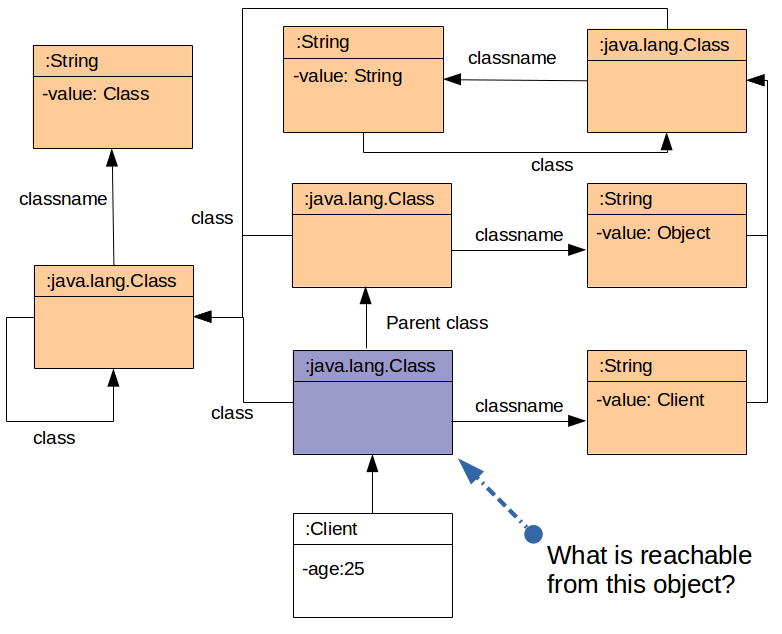
\includegraphics[scale=0.5]{./chapter6/fig/example1.png}
\caption{Objects reachable from the Client class. Observe that only one object is not reachable.}\label{fig:reachable-from-class-object}
\end{figure}

The aforementioned informal steps show what a profiler should be capable of doing:

\begin{itemize}
\item \textbf{Accessing meta-data of objects} such as the class of an object (\textit{java.lang.Class}), and the size of an object. 

\item \textbf{Accessing the value of attributes} is also helpful to filter out elements of the heap.

\item \textbf{Traversing references} is necessary because often some objects belong to a structure only because they are referenced by an object that is already a member.
\end{itemize}

To summarize, a function to determine whether an object is member of an structure may use: properties of the object itself, and properties about its relationships.

%\paragraph{Is there an instance of A making reference to an object of type B?}

%\paragraph{Length of each string, and number of objects referencing each string}

\paragraph{Nodes in each simply linked list}

In a second example, we want to calculate how many nodes has each simply linked list in the heap.
Figure~\ref{fig:simple_snapshot} shows a heap with two simply linked list and one double linked list.
The first list has three nodes while the second one has four; these are the values we want to obtain.

%Mostrar como hay patrones similares que se pueden detectar muchas estructuras
%Que entonces lo que se hace es describir el tipo de estructura con un paramtero adicional.

\begin{figure}[!ht]
\centering
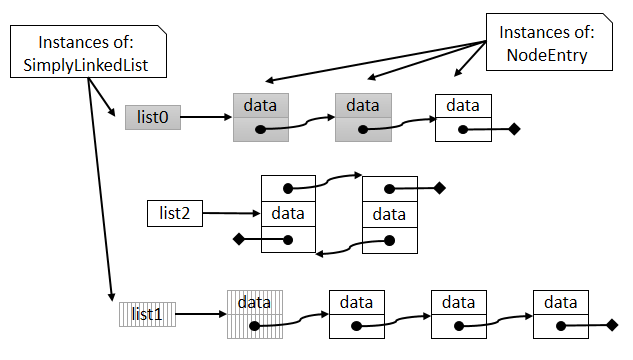
\includegraphics[width=0.65\linewidth]{chapter6/fig/lists}
\caption{Memory snapshot with three linked lists}
\label{fig:simple_snapshot}
\end{figure}


Informally, to compute such data a profiler must traverse the heap, checks whether an object's class is \textit{NodeEntry} (membership function), and increases a counter every time an instance is found (function to compute memory profile).
Unfortunately, these two steps are insufficient to correctly compute the fact that there exist two lists.
Indeed,  instead of the two values 3 and 4, a single value -- seven -- is obtained when this procedure is used.
The problem is that we have two structures instead of one, but using the aforementioned membership function it is impossible to know of which structure an instance of \textit{NodeEntry} is member of.
In other words, we need additional information to distinguish the two structures.

A method to solve this particular problem is to use the following recursive membership function: an object is member of a structure $S$ if it is an instance of \textit{NodeEntry} and it is being referenced by a member of $S$.
For the non-recursive case, we can see how each simply linked list starts with an instance of \textit{SimplyLinkedList}.
This is easily represented with a parametrized and recursive membership function:

\[
	f_{head}\left(O\right) = 
	\begin{cases}
		head = O & \quad O \; is \; \operatorname{SimplyLinkedList} \\
		\exists {x \in \operatorname{Objects}}, \quad x \operatorname{references} o \wedge f_{head}\left(x\right) & \quad O \; is \; \operatorname{NodeEntry} \\
		\operatorname{false} & \quad \operatorname{otherwise} \\
	\end{cases}
\]

The parameter $\textit{head}$ represents the structure of interest, and it is an instance of \textit{SimplyLinkedList}.
In this example, we have two functions, in which only the parameter varies, because there are two instances of class \textit{SimplyLinkedList}.
Similarly, we need two counters to store the number of nodes while we are traversing the graph of objects; once again, they (and the function to compute their values) are parametrized by the $head$ of the list.
Figure~\ref{fig:simple_snapshot} depicts a snapshot in time of the heap while it is being explored;
the shaded nodes are those that were already explored.

This example shows that in defining memory profilers, we often need the capacity for:

\begin{itemize}
\item Using the same functions for many structures, varying only some parameters. This is necessary for both membership functions and to compute the memory profile.

\item Identifying structures in the heap by using a parameter. For instance, in this example, we know that there are two structures because there are two instances of class \textit{SimplyLinkedList}.
\end{itemize}

To summarize, we are frequently interested in calculating values for many structures that have the same ``characteristics''; this is what we call \textit{structure type}.
To identify such structures we use a \textit{parameter}; the process of associating a particular parameter value to a structure type is done by a \textit{factory of structures}. 

\section{Metalanguage to define custom memory profilers}\label{sec:approach}

In this chapter, we propose a tool to create custom memory profilers for MRTEs.
We are interested on easing the task of defining new profilers without sacrificing their performance regarding CPU consumption.
This section presents our approach, a metalanguage to define custom memory profilers in MRTEs.
First, we present a global view of how our approach is used to support resource-aware programming, and how it integrates in a production environments (see Section~\ref{sec:dsl-global-architecture}).
Afterwards, the abstract syntax of this metalanguage is discussed; we present it using a metamodel of its main concepts as well as some snips of code in a concrete syntax to ease the presentation (see Subsection~\ref{sec:abstract-syntax}).
This concrete syntax is then presented in Subsection~\ref{sec:concrete-syntax}, followed by both the operational (evaluation) and translational semantic of the language (see Subsections~\ref{sec:operational-semantic} and~\ref{sec:translational-semantic}).
The section ends in Subsection~\ref{sec:dsl-usage-examples} by presenting some examples of how to use the language.

%Keeping the profiler's overhead as low as possible is of utmost importance for us because lightweight profilers can be use both during the development phase and during the application execution in a production environment.
%To reach this goal, we propose a Domain Specific Language (DSL) and its code generator which aims at describing and generating efficient online memory profilers. 

%We next present the syntax, semantics and usage examples of our domain-specific language.


\subsection{Global Architecture}\label{sec:dsl-global-architecture}

The global architecture of our approach is shown in Figure~\ref{fig:dsl-global-view}.
Since our goal is to support resource-aware programming, in this architecture, an application is able to collect data on its own memory consumption.
To provide this feature, we add a layer (data collection layer) to MRTEs to take care of: 

\begin{itemize}
\item Providing a set of interfaces to the memory profilers for collecting meta-data of objects in the heap, mechanisms to iterate over such objects, and to read the value of their fields.

\item Providing a set of interface for accessing memory profilers from the applications.
In other words, an application may trigger the execution of a memory profiler, and it can analyze the values compute by the profiler.

\item Supporting dynamic loading of memory profilers.
This is helpful in production environment for loading new dynamic analysis tools without having to stop the MRTE.
\end{itemize}

\begin{figure}[!ht]
\centering
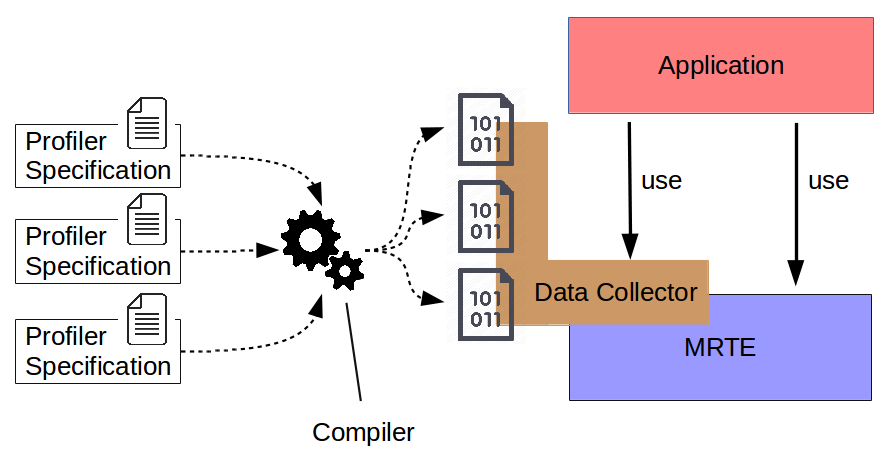
\includegraphics[scale=0.4]{./chapter6/fig/global-view.png}
\caption{Global view of the system. In this case, three memory profilers are defined.}\label{fig:dsl-global-view}
\end{figure}

In Figure~\ref{fig:dsl-global-view}, three memory profilers are plugged to the data collection layer.
The exact mechanism to collect raw data from the MRTE, as well as the mechanisms to dynamically load profilers, are platform specific.

A memory profilers can be handcrafted and plugged in this architecture; this is, nevertheless, error-prone.
Instead, we favor a generative approach where profilers are written using a metalanguage that hides low-level details.
A compiler is then used to transform such definitions into a binary form that can be executed in the runtime environment.
It is also in charge of providing interoperability between the data format provided by low-level facilities of the MRTE, and the high-level data format expected by applications running on top of such execution environments. 

\subsection{Abstract Syntax}\label{sec:abstract-syntax}

The metamodel shown in Figure~\ref{fig:as} describes the abstract syntax of our DSL.
The main concept of this metamodel is a \textit{CustomProfiler} which is composed of \textit{UserDefined} types and a \textit{StructureFactory}.
The concepts related to \textit{UserDefined} types are shown on the left part of the metamodel, while the right part describes the \textit{StructureFactory} which represents both the set of  structures to identify and the value to compute on these structures.

\subsubsection{User-defined types}
In addition to various \textit{BasicTypes} such as \textit{Integer}, \textit{String} and \textit{Boolean}, the language supports the definition of both \textit{Records} and \textit{Lists}.
As expected, a \textit{record} contains \textit{fields} to hold values of previously defined types.
Likewise, a \textit{list} refer to a \textit{base type}; hence all the members of a list must be of the same type.
In a custom profiler, \textit{UserDefined} types can be composed in arbitrary ways as long as no type contains a recursive declaration.
We can formalize such a constrain using OCL (Object Constraint Language~\footnote{\url{http://www.omg.org/spec/OCL/}}):

\begin{lstlisting}[escapeinside={(*}{*)},
label=fig:membership,
language=OCL1
]
context Record inv: 
   not fields->oclAsSet()->closure(t)->exists(t | t = self)

context List inv:
   not baseType->oclAsSet()->closure(t)->exists(t | t = self)
\end{lstlisting} 

A \textit{List} has operations to manipulate any value which represent a list.
Figure~\ref{fig:as} shows a subset of these operations.
In general, these operations correspond to the set of \textit{standard} operations of any implementation of the list data type.

\subsubsection{Defining structures to profile}
Defining the \textit{StructureFactory} is the core of writing a custom profiler.
A \textit{StructureFactory} contains an \textit{Expression} through the \textit{instances} relationship which indicates a pattern to identify structures in the memory heap.
Notice that a single instance of \textit{StructureFactory} creates many data structures in memory; thus the \textit{Expression} corresponds to a list indicating that a new structure must be instantiated for each element of the list.
Forcing the \textit{Expression} to be a \textit{List} can be easily formalized using OCL:

\begin{lstlisting}[escapeinside={(*}{*)}, label=fig:instances, language=OCL1]
context StructureFactory inv: instances.type.oclIsTypeOf(List)
\end{lstlisting}

Defining a new \textit{StructureFactory} implies defining its \textit{type} which is an instance of \textit{StructureType}.
This concept describes the mechanism used to populate, out of objects, a structure and its information.
In short, each structure in memory instanciated through a \textit{StructureFactory} has a type \textit{StructureType}.
For example, we may be interested in finding all the \textit{SimplyLinkedList} in the memory snapshot depicted in Figure~\ref{fig:simple_snapshot}.
In such a case, there are two \textit{SimplyLinkedList}, but we only need one mechanism to identify them because they have the same pattern in memory. 

\begin{figure*}
\centering
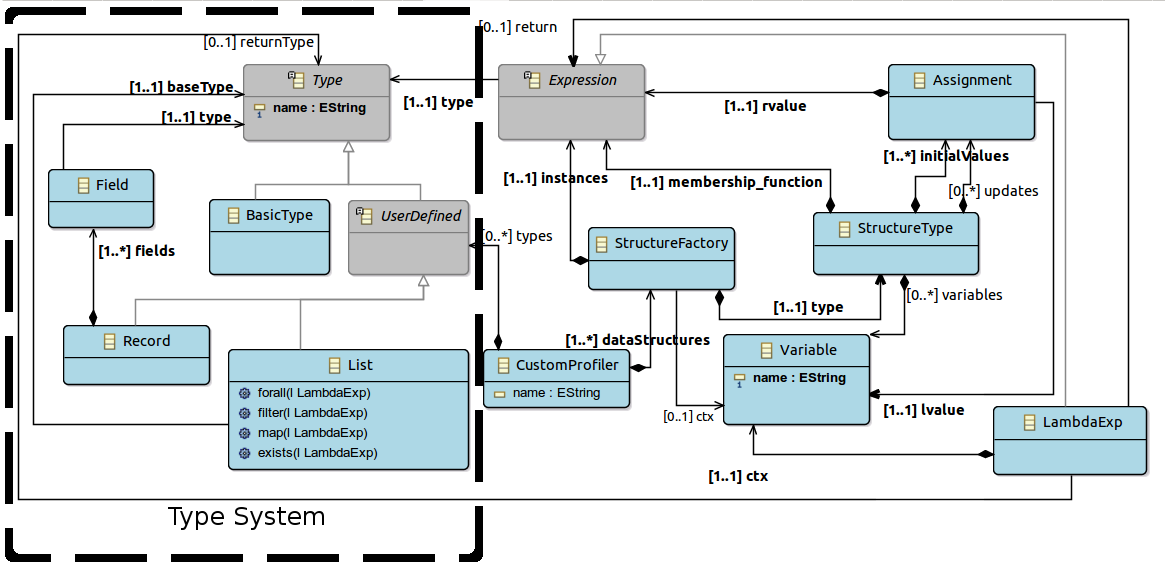
\includegraphics[width=0.87\linewidth]{chapter6/fig/AS}
\caption{Custom profiler Metamodel}
\label{fig:as}
\end{figure*}


A \textit{StructureType} is composed of \textit{Assignments} that are used as \textit{initialValues} for each \textit{Variable} holding information - similar to a constructor in object-oriented programming.
Once a new structure is created, the \textit{Assignments} are executed to assign the initial value of each \textit{Variable}.
Observe that \textit{variables} do not refer to a \textit{Type}.
Our DSL is strongly typed and the \textit{type} of each user-defined variable is inferred from its initial value.
Nevertheless, there is a built-in variable in each \textit{StructureType} that is only accessible during initialization.
Its type is predetermined as part of the language specification.
We force the use of the proper type using OCL:

\begin{lstlisting}[escapeinside={(*}{*)}, label=fig:instances, language=OCL1]
context StructureType inv:  initialValues->exists(a: Assignment | 
     a.lvalue.name = 'initialObjects' and a.rvalue.type.oclIsTypeOf(List)
   ) 
\end{lstlisting}

In addition, a \textit{StructureType} contains a boolean \textit{expression} which is the \textit{membership function} used to decide whether an object should be included in the structure instance.
Finally, it also contains a set of \textit{Assignments} to update the value of each \textit{variable} every time a new object is included in the structure.
This set of \textit{Assignments} is used to compute the actual value of the memory profile.
The major constraint regarding these \textit{updates} is that they must refer to already initialized \textit{variables} and the new assigned values must match the previous types.
We formalize such a constrain using OCL:

\begin{lstlisting}[escapeinside={(*}{*)}, label=fig:lvalue, language=OCL1]
context StructureType inv:  updates->forAll(a: Assignament | 
    self.initialValues->exists(aa : Assignament | 
       aa.lvalue = a.lvalue and aa.rvalue.type = a.rvalue.type
     ))
\end{lstlisting}

In our DSL, \textit{expressions} play a big role.
For the sake of readability, Figure~\ref{fig:as} only shows a couple of concepts related to them.
However, it is noteworthy that, in addition to \textit{arithmetic}, \textit{boolean} and \textit{literals} for basic types, the language includes lambda expressions, literal for records and lists.
Moreover, the language defines \textit{built-in rvalues} which are nothing but expressions initialized by the runtime within a specific scope.
Instead of being user-defined, the types of these expressions are also defined by the runtime.
There are two types of \textit{built-in rvalues}, target independent and dependent.
Among the firsts, we have the list of  \textit{objects}, a reference to the \textit{current data structure} and a reference to the \textit{current object}.
Target dependent \textit{rvalues} in Java include the list of \textit{loaded classes} and the list of \textit{threads}.
The precise meaning of these \textit{rvalues} as well as their scopes are precisely discussed in sections~\ref{sec:concrete-syntax}, ~\ref{sec:semantic} and~\ref{sec:implementation} along the concrete syntax, the language semantic and the tooling support.

Finally, if we use the memory snapshot depicted in Figure~\ref{fig:simple_snapshot}, calculating the number of nodes belonging to a specific \textit{SimplyLinkedList} is an example that illustrates the language's concepts.
To solve this problem we can instantiate the metamodel of our DSL as follow:
\begin{itemize}
\item Define a \textit{StructureFactory} in which the \textit{instances} property is a list which contains the objects \textit{list0} and \textit{list1}.
\item Instantiate a \textit{StructureType} where the built-in variable \textit{initialObjects} receives as value a list with one member - list0 or list1.
      The other properties of this \textit{StructureType} instance are detailed in the next steps: 
      \begin{enumerate}
      \item Define a variable \textit{n} with initial value zero.
      \item Define a membership function which return true if an object is instance of \textit{NodeEntry} and it is referenced by an object for which the membership function also return true. Observe how this recursive function returns true for each element in \textit{list0} because the initial object's list contains object \textit{list0}. 
      \item Update the variable \textit{n} by increasing its value by one.
      \end{enumerate}  
\end{itemize}
Further details about this example are discussed in the next section.

\subsection{Concrete Syntax}\label{sec:concrete-syntax}

A textual concrete syntax has been defined for our DSL allowing the domain expert to define a custom memory profiler using a text editor.
A high-level view of the grammar for this textual representation is depicted in Figure~\ref{fig:dsl-grammar}.
As can be seen, the rules that represent expressions make such a grammar ambiguous, we decided to use this form for the sake of the presentation.
However, a complete LL(*) grammar~\cite{Parr:2011:LFA:1993498.1993548} is presented hereafter in Annex~\ref{anx:grammar}.
One interesting aspect of this concrete language is its relative verbosity.
For instance, it uses very explicit keywords such as ``create structure foreach'', ``constructor'', and ``membership''.


%\setlength{\grammarparsep}{20pt plus 1pt minus 1pt}
{
\scriptsize
\begin{figure}[!ht]
\begin{mdframed}[outermargin=0.2cm, innermargin=0.5cm]

\newcommand{\grule}[1]{\hfill{\scriptsize (#1)}}
\setlength{\grammarindent}{5em}
\begin{grammar}

<program> ::= <types> <structures> \grule{1}

<types> ::= <type> <types> | <empty> \grule{2, 3}

<type> ::= <id> `:' `table-of' <id> | <id> `:' `struct' `{' <fields> `}' \grule{4, 5}

<fields> ::= <id> `:' <id> <fields> | <id> `:' <id> \grule{6, 7}

<structures> ::= <struct-factory> <structures> | <struct-factory> \grule{8, 9}

<struct-factory> ::= `create structure foreach' <id>`:'<e> `using' <body> \grule{10}

%<Header> ::= `create structure foreach' <id>`:'<expr>

<body> ::= `constructor' <s> `membership' <expr> `updates' <s> \grule{11}

%<constructor> ::=  \grule{12}

%<membership> ::= 

%<updates> ::= \grule{13}

<s> ::= <a> <s> | <empty> \grule{12}

<a> ::= <id> `=' <e>  \grule{13} 

<e> ::= <e> <binary-op> <e> | <unary-op> <e> \grule{14, 15}
\alt <e> `in' <id> | <e> `is' <id> \grule{16, 17}
\alt <e> `.' <id> `(' <expr-list> `)' \grule{18}
%\alt <e> `.' <id> `(' `[' <id> `|' <s> `]' `)' \grule{19}
\alt <e> `.' <id>                              \grule{20}
\alt `#[' <expr-list> `]' | `struct' <id> `{' <expr-list> `}' \grule{21, 22}
\alt <int-literal> | <string-literal> | <bool-literal> \grule{23, 24, 25}
\alt <id> | `(' <e> `)' \grule{26, 27}

<expr-list> ::= <e> `,' <expr-list> | `[' <id> `|' <s> `]' `,' <expr-list> | <empty>  \grule{28}

<binary-op> ::= `+' | `*' | `-' | `/' | `and' | `or'

<unary-op> ::= `-' | `not'

\end{grammar}
\end{mdframed}
\caption{Concrete grammar of the language. For the sake of clarity, we are using an ambiguous grammar to describe the expression language.} \label{fig:dsl-grammar}
\end{figure}
}

As an example, the next listing shows how to compute the length of each \textit{SimplyLinkedList} in the memory snapshot depicted in Figure~\ref{fig:simple_snapshot}.
The mechanism is based on counting the number of \textit{NodeEntry} referenced by the \textit{SimplyLinkedList}.
Each \textit{NodeEntry} is used to wrap one element of data and to point to the next element.

\begin{lstlisting}[escapeinside={(*}{*)}, 
label=lst:listLengt, language=DSL2
]
create structure foreach e:objects.filter(l| l is SimplyLinkedList) using
  constructor
    initialObjects = #[e] // a list literal with one element: e
    n = 0
  membership (this is NodeEntry) and (referrer in this_structure)
  updates 
    n = n + 1
\end{lstlisting}

In the example, only one \textit{StructureFactory} is necessary.
In line 1, we define the list of structures we are interested in.
We do so by selecting instances of class \textit{SimplyLinkedList} as elements of the \textit{StructureFactory}.
Since there are two simply linked lists in the memory snapshot, we are going to build two structures.
Observe the usage of a built-in \textit{rvalue} named \textit{objects} which contains all the objects in memory.
The valid scope of this rvalue is in both the definition of the set of structures and the computation of the initial values.
Thereafter, lines 2-4 specify the initial values.
Line 3 in particular initializes the set of objects included in the structure.
Notice the usage of a list literal to include the object referenced by \textit{e}.
In the initialization scope, the rvalue \textit{e} is equal to one of the element within the list of structures - either \textit{list0} or \textit{list1}.

In line 5 we define the membership function, which is used to determine if an object is part of the structure.
There are four built-in rvalues during the evaluation of the function as well as during the update of the variables.
First, the value named \textit{this} is the current visited object. 
The \textit{membership} boolean \textit{expression} aims at determining if this object is part of the \textit{structure} or not. 
The value \textit{this\_structure} identifies the structure.
As our runtime profiler will traverse the graph of in memory objects following references between objects, the object through which we have reached the \textit{this} object is known as \textit{referrer}.
The last value, which is target dependent, is the kind of reference.
Operator \textbf{is} checks if \textit{this} is an instance of class \textit{NodeEntry}.
Likewise, operator \textbf{in} checks whether the \textit{referrer} is already a member of the structure.
Finally, line 7 updates the length of the list when an object is detected as member of the structure.

\subsection{Operational Semantics} \label{sec:operational-semantic}

\extracomment{TODO}{
\begin{enumerate}
\item Add notation
\item Fix the rule that calls a method with a lambda expression
\item Add the rule for the interpretation of a program
\item Discuss the inference rules
\end{enumerate}
}

\begin{figure}
\begin{mdframed}[innermargin=0.3cm, outermargin=0.3cm]

{
\footnotesize

\begin{tabular}{rcl}
$Bool(1)$ and $Bool(0)$ & & \parbox{8cm}{Values  $true$ and $false$.}\\
& & \\
$ E $ & \parbox[t]{0.7cm}{} & \parbox{8cm}{Describes a mapping from \textit{identifiers} to \textit{locations}. We use $id \mapsto l$ to represent a member of the mapping} \\ 
& & \\
$ S $ & & \parbox[t]{8cm}{Describes a mapping from \textit{locations} to \textit{values}. Informally, it can be seen as the storage. We use $l \mapsto v$ to represent a member of the a mapping.} \\ 
& &  \\
$ C $ & & \parbox[t]{8cm}{Describes a mapping from \textit{values} to \textit{structures}. We use $v \mapsto s$ to represent a member of the mapping.} \\ 
& & \\
$\left[ k_1 \mapsto v_2, \dots, k_n \mapsto v_n \right]$ & & \parbox[t]{8cm}{Describes a mapping by enumerating its members.} \\ 
& & \\
$S\left[ v_i/k_i \right]$ & & \parbox[t]{8cm}{Describes a new mapping where $S\left[ v_i/k_i \right](k_j) = S(k_j)$ if $k_i \ne k_j $, $S\left[ v_i/k_i \right](k_j) = v_i$ otherwise. } \\
& &  \\
$M \overset{\operatorname{val\_of}}{\vdash} k \mapsto v$ & & \parbox[t]{8cm}{A set of auxiliary rules to compute the value $v$ that is associated to the key $k$ in the mapping $M$.} \\ 
& &  \\
$C \overset{\operatorname{contains}}{\vdash} v \mapsto s \Rightarrow r$ & & \parbox[t]{8cm}{A set of auxiliary rules to determine whether the value of $v$ is mapped to $s$ in $C$, which is always a mapping from  \textit{values} to \textit{structures}. $r$ is a boolean value. } \\
& &  \\
$\lVert E,S, id, e\rVert$ & & \parbox[t]{8cm}{Describe a closure, $E,S$ represents the state, $id$ is the identifier used as parameter of the closure, and $e$ is the expression to evaluate.} \\ 
& & \\
$T(a_1 \mapsto l_1, \dots, a_n \mapsto l_n)$ & & \parbox[t]{8cm}{A generic value in the language. $T$ is its type, and a mapping from attributes $a_i$ to their respective locations $l_i$. Sometime, we use $\mathbb{A}$ to represent the mapping. There are shorthands for special cases: $Bool(1)$, $Bool(0)$, $Int(n)$ which is the integer $n$, and $String(w)$ which is the string $w$. In addition, the value $table(l_1,\dots,l_n)$ denotes a table; in this case, $l_i$ is the location in storage of the \textit{i-th} element of the table. } \\ 
& & \\
$\langle T, P, a_1 \mapsto T_1, \dots, a_n \mapsto T_n \rangle$ & & \parbox[t]{8cm}{Describe a type with identifier $T$. The description contains the parent type $P$ (which has the same structure), and its attributes $a_i \mapsto T_i$. } \\
& & \\ 
$\overset{\operatorname{subtype}}{\vdash} S, P \Rightarrow r$ & & \parbox[t]{8cm}{A set of auxiliaries rules to determine whether type $S$ is a subtype of $P$. $r$ is a boolean value.} 
\end{tabular} 

}

\end{mdframed}
\caption{Notation used in the operational semantic}\label{fig:notation-for-operational-semantic}
\end{figure}

\renewcommand{\inference}[3][]{%
  \begin{array}[b]{@{}c@{}c@{}}
    \smash{\raisebox{-.5\normalbaselineskip}{{\scriptsize #1}}} & 
      \begin{array}[b]{l}
        #2
      \end{array} \\
      \cline{2-2}
    & \begin{array}[t]{c}
        #3
      \end{array}
  \end{array}
}

\mathlig{->}{\mapsto}
\mathlig{|-}{\vdash}
\mathlig{=>}{\Rightarrow}
\mathlig{"}{\;\;\;}

\mathligson

% classics
{
\footnotesize
\[
% true
\textnormal{{\scriptsize It(25):}}\; E, S\vdash\operatorname{true}\Rightarrow Bool(1),S
\quad\quad
% false
\textnormal{{\scriptsize It(25):}}\; E, S\vdash\operatorname{false}\Rightarrow Bool(0),S
\]

\[
% integers
\textnormal{{\scriptsize It(23):}}\; E, S\vdash\operatorname{Integer}\; N\Rightarrow Int(N),S
\quad\quad
% strings
\textnormal{{\scriptsize It(24):}}\; E, S\vdash\operatorname{String}\; w\Rightarrow String(w),S
\]

% lambda expressions
\[
\textnormal{{\scriptsize It(19):}}\; E, S\vdash \left[id \vert e \right] \Rightarrow \lVert E,S, id, e\rVert,S
\]

\[
% id
\inference[It(26):]{
E\overset{val\_of}{|-}id->l_{id} "" S\overset{val\_of}{|-}l_{id}->v
%v = S \; E \; id
}{E, S|-id=>v,S}
\quad\quad
% (e) 
\inference[It(27):]{
E, S|-e=>v,S_1
}
{E, S|-(e)=>v,S_1}
\]

\[
% unary operators
\inference[It(17b):]{
E, S|-e_0=>v_0,S_1
}{E, S|-\operatorname{op}e_0=>\operatorname{op}v_0,S_1}
\quad\quad
% binary operators
\inference[It(17a):]{
E, S|-e_0=>v_0,S_1 "" E, S_1|-e_1=>v_1,S_2
}{E, S|-e_0\operatorname{op}e_1=>v_0\operatorname{op}v_1,S_2}
\]

\[
% in operator
\inference[It(17c):]{
C, E, S|-e_0=>v_0,S_1 "" C \overset {in} {|-} v_0->id =>v
%v = v_0->id \in C? Bool(1):Bool(0)
}{C, E, S|-e_0 \; in \; id=>v,S_1}
\quad\quad
\]

\[
% is operators
\inference[It(17d):]{
E, S|-e_0=>X(\mathbb{A}),S_1 "" \overset{subtype}{|-} X, T \Rightarrow v
}{E, S|-e_0\; \operatorname{is} \; T:v,S_1}
\]

\[
% assignment
\inference[It(16):]
{
E,S|-e_0=>v_0,S_1 "" E\overset{val\_of}{|-}id->l_{id}
%l_{id} = E(id) \\
%S_2 = 
}
{E, S|-id = e_0=>v_0, S_1[v_0/l_{id}]}
\quad\quad
% statements
\inference[It(14)]
{
E, S|-a=>v_a,S_1 "" E, S_1|-s=>v,S_2
}
{E, S|-a\;s=>v,S_2}
\]

\[
% struct literal
\inference[It(22):]
{
E,S|-e_1=>v_1,S_1 \\
\vdots \\
E,S_{n-1}|-e_n=>v_n,S_n \\
\operatorname{class}(T)=(a_1->T_1, \dots, a_n->T_n) \\  % take the fields of the object
l_i = \operatorname{newloc}(S_n) \; for \; i = 1 \dots n \\
v=T(a_1->l_1, \dots, a_n->l_n) \\ % assign locations to fields
S_f = S_n[v_1/l_1, \dots, v_n/l_n]
}
{E, S|-struct\;T\;\{ e_1, \ldots, e_n \}:v,S_f}
\quad\quad
% list literal
\inference[It(21):]
{
E,S|-e_1=>v_1,S_1 \\
\quad \vdots \\
E,S_{n-1}|-e_n=>v_n,S_n \\
l_i = \operatorname{newloc}(S_n) \; for \; i = 1 \dots n \\
v=\operatorname{table}(l_1, \dots, l_n) \\
S_f = S_n[v_1/l_1, \dots, v_n/l_n]
}
{E, S|-\#[e_1, \dots, e_n]:v,S_f}
\]

\[
% accessing field
\inference[It(20):]{
E,S|-e=>X(\mathbb{A}),S_f "" \mathbb{A} \overset{val\_of}{|-} \textit{id} -> l_{\textit{id}} "" \mathbb{S} \overset{val\_of}{|-} l_{\textit{id}} -> v
%v0 = X(a_1->l_1, \dots, a_n->l_n) \\
%l_{id} = l_i \; where \; a_i = id \\
%v = S_1(l_{\textit{id}}) \\
}
{E,S|-e.\textit{id}=>v,S_f}
\]

\[
% calling method
\inference[It(18):]{
E,S|-e_0=>X(\mathbb{A}),S_0 \\
E,S_0|-e_1=>v_1,S_1 \\
""" \vdots \\
E,S_{n-1}|-e_n=>v_n,S_n \\
\operatorname{impl}(X,f) = (x_1, \dots, x_n, f_{body}) \\
l_{x_i} = \operatorname{newloc}(S_{n+1}) \; for \; i = 1 \dots n \\
\mathbb{A}[l_{x_1}/x_1, \dots, l_{x_n}/x_n],S_n[v_1/l_{x_1}, \dots, v_n/l_{x_n}]|-f_{body}:v,S_f
}
{E,S|-e_0.f(e_1, \dots, e_n):v,S_f}
\]

% news

%\[
%% lambda expressions
%\inference[It(19) mal]{
%v = \lVert E, \left[ id | s \right] \rVert " a " v
%}{
%E,S|-[id|s]:v,S
%}
%\quad\quad
%% calling function with lambda expression
%\inference[It(19) mal]{
%E,S|-e_0:v_0,S_1 \\
%v_0 = X(a_1=l_1, \dots, a_m=l_m) \\
%\operatorname{impl}(X,f) = (x_1, f_{body}) \\
%l_{x_1} = \operatorname{newloc}(S_1) \\
%E' = [a_1:l_1, \dots, a_m:l_m][l_{x_1}/x_1] \\
%v_1 = \operatorname{Clousure}(E, \left[ id | s \right]) \\
%v_0, E', S_1[v_1/l_{x_1}]|-f_{body}:v,S_f 
%}{
%E,S|-e_0.f\left( \left[ id | s \right] \right):v,S_f
%}
%\]
%
}



\mathligsoff

\subsection{Translational Semantics}\label{sec:translational-semantic}

An instance of our metamodel is compiled into a custom memory profiler.
This compilation produces a library written in \textit{C++} which is in charge of collecting the desired information from the runtime environment.
The generated source code has two parts.
First, for each \textit{StructureType} in the model, the compiler generates a subclass of \textit{AbstractStructureType} which is shown below.
Every subclass contains attributes to store the variables used in the associated \textit{StructureType}.
In the listing below, the class \textit{Context} holds the built-in values we mention in the previous section.
\begin{lstlisting}[language=C++, frame=L,
numbers=left,
numberstyle=\color{black}\scriptsize,xleftmargin=2\parindent]
class AbstractStructureType {
public:
	void initialize(Context& ctx) = 0;
	bool membership(Context& ctx) = 0;
	void update(Context& ctx) = 0;
}
\end{lstlisting}

The second part of the generated code is formed by a set of initialization routines, one for each \textit{StructureFactory}.
Each routine creates a list of structures with a specific \textit{AbstractStructureType} - the \textit{T} parameter in the listing.
Formally, the signature and behavior of these routines are as follow:
\begin{lstlisting}[language=C++, frame=L,
numbers=left,
numberstyle=\color{black}\scriptsize,xleftmargin=2\parindent]
template <typename T> void
[name](Context& ctx, std::vector<AbstractStructureType*>& s){
  for (Object obj : ctx.instances) {
    AbstractStructureType* ns = new T();
    ctx.e = obj;
    ns->initialize(ctx);
    s.add(ns); // not valid in the STL, but simpler to read
  }
}
\end{lstlisting}
An important concern during the transformation lies on efficiently mapping our concepts to \textit{C++} concepts.
Moreover, since each target platform provides facilities to get metadata regarding the objects in memory, using such facilities efficiently is specially important in order to reduce the performance overhead due to profiling.

The final profiler is built using both the generated code and a template algorithm.
The template is target dependent, but in general we use the underline target facilities to collect meta-data, access fields in certain steps, traverse the objects in memory and also to populate the built-in rvalues.
A simplified version of the used algorithm is shown below:
\begin{lstlisting}[escapeinside={(*}{*)},
label=lst:template, language=AlgLang, frame=L,
numbers=left,
numberstyle=\color{black}\scriptsize, xleftmargin=2\parindent]
values:
   structures: vector<AbstractStructureType*>
routine:
   foreach (initialization rountine (*$R_i$*) associated to a StructureFactory)
      create context
	  call (*$R_i$*)(context, structures)
   foreach (r: references among objects)
      if (r.target has no membership)
         create context // context.this = r.target
         S = structures.findfirst(s | s.membership(context))
         make context.this a member of S
         S.update(context)
   return structures 
\end{lstlisting}
There are two loops in the algorithm. 
The former loop is in charge of creating the set of structures the program is intended to collect information about.
The creation of the context in line 5 depends on the target platform.
It basically creates values such as the list of objects in memory or the list of loaded classes.
The latter loop traverses all the references among objects in memory.
During each iteration, the algorithm finds the first structure for which the membership function is true.
Notice that we only select the first because for some memory accounting problems, it is too hard to define a membership functions that build disjoints structures~\cite{dsn/09/geoffray/ijvm,Attouchi:2014:MMM:2602458.2602467}.
Thereafter, the information for such a structure is updated.

%The complete execution of a program in our language is as follow. Subgraph instances are initialized using listing~\ref{onInitialization}.
%Afterward, all the references in the graph of objects are traversed running listing~\ref{lst:onNodeFoundData}.
%The output data for all subgraph instances has been collected after all the references are traversed once.

%Finally, in listings~\ref{lst:onNodeFound},~\ref{lst:onNodeFoundData} and~\ref{onInitialization} we use built-in properties that are defined by the user.
%These properties must have access to some data describing the content of the memory in order to successfully identify subgraphs and calculate output values.
%Such data is wrapped in what we call execution context.
%In our DSL there are two different execution contexts: \textit{global context} and \textit{local context}.
%The former includes built-in values such as: i) lists of \textit{objects}, \textit{threads}, \textit{classes}, etc. , and ii) a value called \textit{Entity} representing a subgraph instance.
%The latter only contains the object \textit{THIS} which is being visited, a label of the reference representing its type, \textit{REFERRER} which is the object referencing the visited and again the \textit{Entity} value.
%The \textit{global context} is available in listing~\ref{onInitialization} while the \textit{local context} is available in both listings~\ref{lst:onNodeFound} and~\ref{lst:onNodeFoundData}.

\subsection{Language Usage} \label{sec:dsl-usage-examples}

\extracomment{FIX}{Improve explanations, add a caption to each listing, improve the style of each listing}

There are several possibilities for using our DSL in the various stage of an application lifecycle.
These include checking: local data structure invariants, reachability properties, memory consumption properties and combinations of those.
Below, we show some examples to highlight possible usage of our language. 
 
The first example shows how to assert the existence of a value satisfying some properties, independently of which object contains it. 
The result is obtained through the use of a filter on the list of objects.
The assertion successes if the heap contains an object with an attribute named $data$ with a value comprised between $3.141$ and $3.142$.

\begin{lstlisting}[escapeinside={(*}{*)},
%label=assertion, 
language=DSL2]
create structure foreach e:#["whole-jvm"] using
  constructor
    initialObjects = #[]
    existValue = false
  membership true
  updates 
    existValue = existValue or (this.data > 3.141 and this.data < 3.142)
\end{lstlisting}

The goal of next listing is to detect a bug identified in~\cite{Aftandilian:2009:GAU:1543135.1542503}.
This listing aims at finding if there exists an instance of the class $Order$
with the value of its field $field$ being equal to $specialValue$.
This technique is used to detect if one object has been garbage collected or if someone still holds a reference on it preventing its garbage collection.

\begin{lstlisting}[escapeinside={(*}{*)},
%caption=Detecting a knwon bug in pseudojbb., 
%label=pseudojbb,
%float=!h,
language=DSL2]
create structure foreach e:#["whole-jvm"] using
  constructor
	initialObjects = #[]
	fault = false
  membership  true
  updates
    fault = fault or (this is Order and this.field = specialValue)
\end{lstlisting}

The next example computes a combination of reachability and memory consumption properties.
It calculates the number of objects, and their total memory consumption, that are reachable from the threads.
We can notice how the membership property discards those objects that are not referenced by an already included object.  

\begin{lstlisting}[escapeinside={(*}{*)},
caption={Calculating objects reachables from threads},
label=kevoreeaccounting,
%float=!h,
language=DSL2]
create structure foreach e:#["whole-jvm"] using
  constructor
    initialObjects = threads
    nbObjects = 0 
    nbSize = 0 
  membership ( this in None and referrer in this_structure )
  updates 
    nbObjects = nbObjects + 1  
    nbSize = nbSize + this.size
\end{lstlisting}

We can also express complex structures in memory.
For instance, to find the consumption of K3-Al object namely \textit{K3Object} as described in Section~\ref{sec:chapter2-introduction}, we must find all instances of \textit{HashMap.Entry} that have \textit{K3Object} as the \textit{key}. These entries should be added to the consumption of the object \textit{K3Object} as well as all the objects reachable from the \textit{HashMap.Entry.value}.
To come out with this solution a good understanding of how K3-Al implements aspects is required.
The rationale here is that K3-Al stores the state of aspects in a separate HashMap, using as key the object to be aspectized.

\begin{lstlisting}[escapeinside={(*}{*)},
%caption=Computing the consumption of each K3-Al Object along with its aspects., 
%label=k3,
%float=!h, 
language=DSL2]
create structure foreach e:objects(*{.filter}*)([it|it is K3Object]) using
  constructor
    initialObjects = #[e]
    nbSize = 0
  membership (referrer in this_structure and this in None ) or
    (this is HashMap.Entry and this.key in this_structure and 
      this.key is K3Object)
  updates
    nbSize = nbSize + 1
\end{lstlisting}

\section{Tooling}\label{sec:dsl-implementation}

To validate our approach, we have implemented a tool chain to ease the definition of custom memory profilers for Java-based systems.~\footnote{Available at: \url{https://github.com/intigonzalez/heapexplorer\_language}}
These profilers can be executed in any JVM as long as it provides support for the JVMTI.

In this section, we present tools built to support the definition of memory profilers using our language; this is done by taking into account how engineers in different roles may interact with these tools and with the resultant profilers.
Indeed, in dealing with memory profilers, we have to take into consideration the two usual roles -- developers of profilers and their users; after all, profilers built using our language are themselves software abstractions.
A developer must know how the target domain-specific abstractions are represented atop the JVM, and she also must have a clear understanding of how our language is executed.
On the contrary, users only need to be aware of the interface provided by our framework, and the structure of the data collected by a profiler.
In the rest of this section, we discuss details that are important to these roles.

Additionally, we present low-level details regarding how the language is implemented atop of the JMVTI.
The decision of implementing our approach by relying on JVMTI has advantages and disadvantages.
On the one hand, the obvious advantage lies on the portability of this solution, which makes it more valuable from a practical point of view.
On the other hand, building profilers on top of the JVMTI, instead of directly modifying the JVM, impacts the performance of the generated profilers and, unfortunately, hinders (in extreme case it even prevents) the implementation of some language constructs.
Nonetheless, it is our belief that guarantying profilers' portability should be of maximum priority.
Moreover, in writing this implementation, we have found that the limitations in the JVMTI preventing the construction of better profilers can be overcome with, at most, a few additions to the API.


\subsection{Developers of domain-specific abstractions}

%\extracomment{FIX}{I am fixing this section, you can continue in Section~\ref{sec:dsl-tooling-users}}

In our vision, developers of software libraries and component frameworks, as well as software language engineers may use our approach to  define customized memory profilers for the abstractions they create.
This is, in addition to delivering artifacts such as libraries, source code, simulators, text editors for DSLs, and compilers for these DSLs; engineers would also ship profilers to simplify the use of these abstractions.
For instance, the developers of the Spring framework~\footnote{\url{https://spring.io/}} may create a set of specific profilers to reduce the cost of maintaining applications written using the framework.
These profilers can serve as both internal tools to help in the development of abstractions, and mechanisms allowing users to better use abstractions.

Figure~\ref{fig:dsl-tooling-developer} summarizes the viewpoint of developers of domain-specific abstractions.
To write a profiler, they use knowledge about the abstraction and the tool chain to generate the executable profiler. 
Our implementation of the language is built using Xtext~\cite{Eysholdt:2010:XIY:1869542.1869625}; it provides a textual editor that is able to handle the proposed concrete syntax.
This editor provides syntax highlighting, error detection during editing, auto-completion, and compilation to native Java agents written in \textit{C++}.

\begin{figure}
\centering
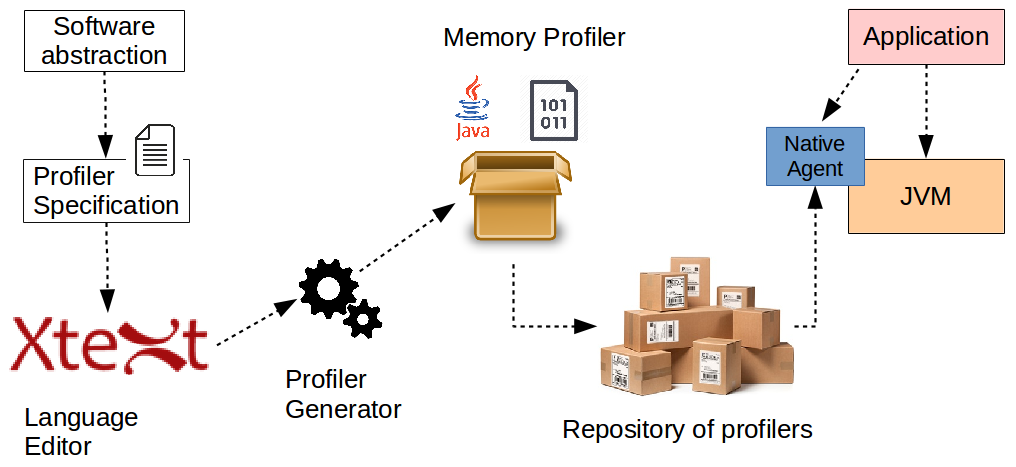
\includegraphics[scale=0.45]{./chapter6/fig/developer-profiler-view.png}
\caption{Viewpoint of developers. Memory profilers are built from the description of software abstractions.}\label{fig:dsl-tooling-developer}
\end{figure}

To perform low-level tasks related to memory profiling, we use \glslink{JVMTI}{JVMTI}~\footnote{\url{http://docs.oracle.com/javase/8/docs/platform/jvmti/jvmti.html}} and \glslink{JNI}{JNI}.
These APIs are used by both profilers and the core memory profiling library, so-called Native Agent in Figure~\ref{fig:dsl-tooling-developer}.
In this native agent, a \textit{plugins} system, which allows users to load/unload profiles without shutting down the JVM, is implemented.
Given a profiler definion, the compiler output is a package that contains a package with the native binary code for the profiler, and a Java library you can use to access the collected data using plain Java objects.

To reduce the overhead of profilers, developers must be aware of the details of the abstraction for which the profiler is being built, the semantic of our language, and the details of its implementation.
In particular, it is advisable reducing the usage of \textit{lists} and the evaluation of nested lambda expressions.
Likewise, heavily using the built-in rvalue \textit{objects} is specially discouraged because it can easily contains many elements.
It is also discouraged because, in order to reduce memory consumption, we rely on an iterator built on top of JVMTI operations that can be costly to use in terms of CPU time.

Finally, we added some built-in rvalues in this implementation because they are both useful in the context of Java and easy to obtain using the JVMTI.
These values are \textit{classes}, \textit{classloaders}, \textit{threads} and \textit{objects}; they are lists of anonymous built-in record types.
The relations among these types and their operations are depicted in Figure~\ref{fig:dsl-built-in-types}.

\begin{figure}
\centering
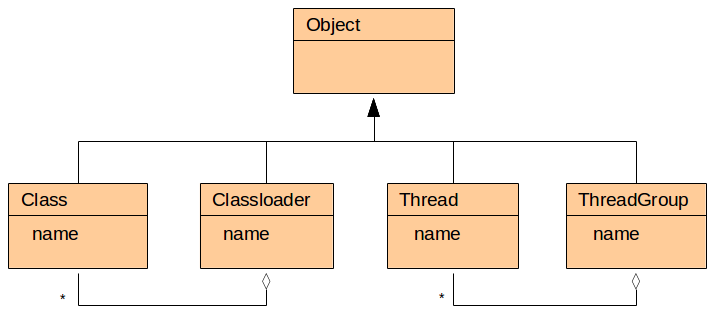
\includegraphics[scale=0.45]{./chapter6/fig/diagram-classes.png}
\caption{Viewpoint of developers. Memory profilers are built from the description of software abstractions.}\label{fig:dsl-built-in-types}
\end{figure}

%Indeed, the process of code generation is driven by the need of reducing the performance impact.
%In our implementation, we apply a set of platform dependent optimizations taking into account the profiler description.
%First, since a profiler does not always need built-in rvalues (e.g., \textit{threads}, \textit{threadgroups} and \textit{classes}, etc.), we selectively skip the construction of them.
%When possible, we also skip the construction of some structures (e.g., class of each object, its classloader, field names, etc.).

\subsection{Users of domain-specific abstractions} \label{sec:dsl-tooling-users}

We envision that a set of memory profilers can be shipped in addition to other ``classic'' deployment artifacts that users of a software abstraction receive. 
These profilers would support the use of the corresponding software abstraction.
For instance, an user who is relying on a new extension of the Xtend language to build a system, might use specific profilers written in our language to understand the memory consumption, and in general, the behavior of the system.

The generated profilers can be used in two different ways, either as development tools or as mechanisms to support resource awareness at runtime.
Due to the scope of this thesis, the reference implementation we provide is biased towards the second scenario, but it should be relatively simple to adapt it to support the software development process.
To access memory profilers, a JVM must be launched with a native Java agent loaded, and a library to collect profiling data in its classpath.
Once the application is running, it can trigger profiling by simple issuing a few method calls using the profiling API.
Figure~\ref{fig:user-profiling-library-view} illustrates the process of collecting memory profiles, the software components involved, and the APIs that must be used.
Observe how the profiling framework issues a call to a handler once it is done, a parameter contains the data computed.
These data are encoded in a \textit{list}, in which each elements correspond to the data computed for each identified structure in the heap.
%The problem is knowing the type and shape of each list element.

\begin{figure}[!b]
\centering
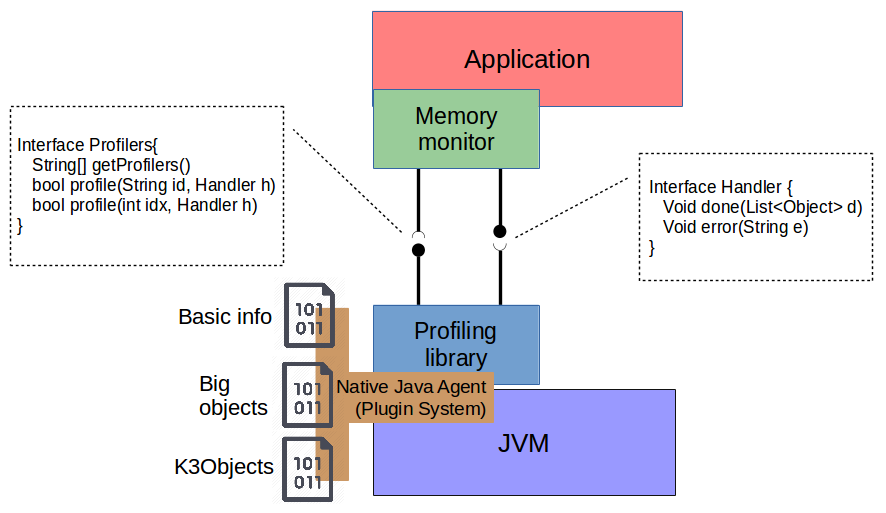
\includegraphics[scale=0.6]{./chapter6/fig/user-profiler-view.png}
\caption{Viewpoint of users. Memory profilers are black-boxes accessed through Java interfaces. Data collected is in the form of plain Java objects.}\label{fig:user-profiling-library-view}
\end{figure}

The output of a profiler is a list of Java objects containing the collected information; and the type of these objects depend on the profiler definition.
Indeed, as part of our implementation, the profiler generator creates a set of Java classes to represent the data collected in a form that is easy to digest at runtime by a Java application.
Once a profiler collects the information in an internal format, it populates a representation in Java using the Java Native Interface (JNI); the code to do so is also generated by the compiler of our language.
In Figure~\ref{fig:dsl-generated-java}, the classes generated for a profiler are shown.
Notice that a class is created for each \textit{record} declared, and also for each \textit{StructureType}.
It can be seen how `lists' are directly represented in Java by mean of generic Java lists.
The \textit{id} field in both \textit{MemoryProfile1} and \textit{MemoryProfile2} is the value used to parametrize each structure;
in this particular example, where two structures are identified, the value of \textit{MemoryProfile1.id} is ``lists'' and the value of \textit{MemoryProfile2.id} is ``otherObjects''.

Given the fact that the data computed by a profiler is returned as a list of objects, and their layout is unclear, the remaining problem is how to process such data; there are two options.
First, users can make the application code depend on the Java code created by the profiler generator.
In this way, your application has a new dependency, but you can profit from knowing at development time the types used in the code.
A second approach is using the reflection capabilities of Java to explore the data.
In the evaluation, we use such an approach to log the result of an arbitrary profiler, printing all the information it has computed.
Using reflection, it is also possible to build a user interface to explore the results in a customized way.  

\begin{figure}
\centering
\begin{minipage}[t]{0.60\linewidth}
\begin{lstlisting}[language=DSL2]
name "basic info" 

T : struct {
	classname : String
	size: int
}
create structeres for e:#["lists"]
using
	constructor
		initialObjects = #Object[]
		data1 = #T[];
	membership
		(this is String) or (this is Array)
	updates
		data1 = data.add(struct T { this.classname, this.size})
		
create structeres for e:#["otherObjects"]
using
	constructor
		initialObjects = #Object[]
		data2 = #T[];
	membership true
	updates
		data2 = data.add(struct T { this.classname, this.size})
\end{lstlisting}
\end{minipage}
\hspace{0.07\linewidth}
\begin{minipage}[t]{0.30\linewidth}
\begin{lstlisting}[language=java, frame=L, numbers=left,numberstyle=\color{black}\scriptsize]
class T {
	final String classname;
	final int size;
}

class MemoryProfile1 {
	final Object id;
	final List<T> data1;
}

class MemoryProfile2 {
	final Object id;
	final List<T> data2;
}
\end{lstlisting}
\end{minipage}
\caption{Representation of profiling data in Java, as users of profilers see it. Accessing these structures is useful to support resource awareness.} \label{fig:dsl-generated-java}
\end{figure}




%The process of code generation is driven by the need of reducing the performance impact.
%In general, there are two ways of optimizing the impact of the memory's analysis.
%First, we can apply platform dependent optimizations.
%The second option is to apply platform independent optimizations; for instance, simplifying the evaluation of each expression.
%In our implementation, we use both platform dependent and independent optimizations.
%
%A set of platform dependent optimizations we perform is related to the construction of the built-in values \textit{threads}, \textit{threadgroups}, \textit{classes}, etc. 
%Since not all memory analysis depends on such values, we selectively skip the construction of them.
%For instance, in listing~\ref{assertion} there is no need to compute any of such values as is also unnecessary to identified the class of each object.
%Extending this idea to other cases (e.g., class of each object, its classloader, field names, etc.) is straightforward.
%To implement these optimizations, we used a parametrized code template, so the code generate depends on the values of these parameters which we can tune to satisfy our needs.
%
%An other optimization we perform is related to the existence of collections as data type in our DSL.
%These collections can be potentially large, in particular, the \textit{objects} value is costly to compute and keep in memory.
%This fact combined with the usage of operations on collections such as \textit{map} and \textit{filter} may harm the performance of an analysis.
%That is why we devise two strategies to deal with collection values.
%User-defined and most built-in collections are kept in memory using linear space.
%On the contrary, we represent the built-in collection \textit{objects} as a generator.
%This representation is feasible because the mechanism provided by JVMTI to access the objects is based on callbacks.
%
%A last optimization is reducing the nodes of the graph that must be traversed
%As an illustration, we only produce code to explore primitive fields of each object, which are represented as leaf nodes in the graph, if there exist some expression accessing a field.
%
%As for platform independent optimizations, we mostly change the order in which boolean expressions are evaluated.
%We try to guarantee that subexpressions accessing collections and fields are evaluated as little as possible.
%
%The current implementation is limited in the number of optimization it applies.
%The main overhead reduction is achieved thanks to the execution model in which many paths of the graph are not traversed.
%Other benefits come from deciding at compilation time if some parts of the graph such as the leaf nodes must be explored or not.


\section{Discussion On Language Expressiveness}\label{sec:expressiveness}

In our DSL, the mechanism used to collect data is explicit to the user.
Hence, it is possible to estimate the overhead of a specific profiler.
In short, our DSL follows the imperative paradigm to obtain derived values.
On the contrary, most query languages provide a declarative style because it \textit{simplifies} writing new queries.

%Designing a domain specific language for memory analysis is a deliberate attempt to make explicit to the user what is the complexity of the analysis he tries to perform.
We acknowledge that our approach limits the kind of memory analysis that users can express.
First, it is not possible to recover all the information contained in the graph of live objects in linear time on the number of objects.
Second, an imperative style forces the users to understand the underlying execution model which is not required with declarative query languages.
Nonetheless, we claim that getting rid of some expressiveness is a trade-off worth considering in order to guarantee efficient memory analysis.
The empirical and theoretical evidence suggest that, in our DSL, \textit{reducing the capabilities to collect data} has a bigger impact on performance gain than \textit{generating efficient native code} to collect data.

At this point, it is worth noting why declarative approaches fail to deliver the adequate performance in production.
Listings~\ref{k3OQL} and~\ref{k3Cypher} show possible solutions, in OQL and Cypher/Neo4j, to the K3-Al example presented in section~\ref{sec:motivation}.
There are two aspects affecting the performance of this kind of queries.
We next discuss them.

\begin{lstlisting}[escapeinside={(*}{*)},caption={Using OQL to compute the consumption of each K3-Al object. Actually, this query cannot be executed in Eclipse Mat nor in VisualVM since they do not provide a full OQL implementation. }, label=k3OQL,float=!h, language=OQL]
SELECT id, sum(size) as s
FROM (
	SELECT
		e.key.@objectId AS id, 
		e.@usedHeapSize + e.value.@retainedHeapSize AS size
	FROM java.util.HashMap$Entry e
	WHERE (classof(e.key).@name = "K3Object")
	UNION ALL
	SELECT 
		k3.@objectId AS id, k3.@retainedHeapSize AS size 
	FROM K3Object k3
)
GROUP BY id
\end{lstlisting}

In the first place, many queries are intrinsically complex to answer.
For instance, it is known that answering SPARQL queries - which was used as inspiration for Cypher/Neo4j, is PSPACE-complete~\cite{Schmidt:2010:FSQ:1804669.1804675, Perez:2009:SCS:1567274.1567278}.
The performance of declarative queries for in production memory analysis is also affected by the nature of data we are exploring. 
Indeed, even if they can be executed efficiently, the optimization steps required are in most cases impossible to execute for the type of data we are considering - a graph of objects that constantly changes.
Often, these query optimizations require access to indexes, additional storage and multiples passes on the data~\cite{Elhemali:2007:ESS:1247480.1247598, Dageville:2002:SMM:1287369.1287454} that are not accessible on the graph of objects.
\begin{lstlisting}[escapeinside={(*}{*)},
caption={Using Cypher to compute the consumption of each K3-A1 object.}, label=k3Cypher,float=!h, language=CYPHER]
MATCH 
	(key:K3Object)<-[:key]-(entry:HashMap$Entry)-[:value]->value
WITH entry, key, value
MATCH 
	key-[:1..1]->fieldK
WITH entry, key, value, fieldK
MATCH 
	value-[:1..1]->fieldV
RETURN key, entry.size + key.size + fieldK.size + sum(value.size) + sum(fieldV.size);
\end{lstlisting}

On the contrary, our language makes explicit both the time and space complexities of the analysis.
We also believe that the mental model required to code profilers with our DSL is simple enough since
we mimic the popular ``think as a vertex'' paradigm of Pregel which has proven to be successful~\cite{Malewicz:2010:PSL:1807167.1807184}.
In this paradigm, an algorithm on graph is described from the point of view of each vertex.
In our case the \textit{membership function} and the \textit{update section} are also executed using a limited context which only includes a few built-in rvalues.

%Finally, we have shown along this paper how to collect meaningful data with ou DSL.
%Nonetheless, it is worth mentioning that the class of common  

%\begin{lstlisting}[escapeinside={(*}{*)},caption=Detecting a knwon bug in pseudojbb., label=pseudojbbOQL,float=!h, language=OQL]
%SELECT o
%FROM Order o
%WHERE o.field = specialValue
%\end{lstlisting}

\section{Evaluating performance of profilers}\label{sec:evaluation}
%\todo{Add research questions}

In this section we evaluate the implementation of our approach with several experiments.
To do so, we present a set of experiments to evaluate the performance overhead of executing different memory analysis.
A goal of this section is to show that our approach induces low overhead across different applications and types of analysis.
Since such analysis exhibit different levels of complexity, we cover a wide spectrum of use even if we are running the experiments with few types of analysis.
%We evaluate the performance of our DSL with several experiments:
 These experiments aim at answering the following research questions:
\begin{enumerate}
\item \textbf{RQ1. Does our approach produce profilers with lower overhead than state-of-the-art tools when used to perform many iterations of memory analysis at runtime?} To answer this question, we assess the overhead on total execution time produced by the periodic computation of a specific analysis.
In this experiment we measure and compare the overhead of our approach against the overhead produced by other solutions.
\item \textbf{RQ2. Is significant the difference between the time needed to execute a single analysis with our approach in comparison to previous solutions? }
In a second experiment, we measure the execution time needed to perform a single memory analysis step instead of focusing on the total application execution time.
\item \textbf{RQ3. Does the advantage of our approach remain for real applications? }
 Finally, we perform memory analysis on actual applications including \textit{Eclipse}, \textit{NetBean} and others to assess the overhead of profiling in ``real life'' scenarios. 
\end{enumerate}

In general, these experiments show that our DSL produces specific profilers with lower overhead for applications running in production environments than well-known memory profilers.

\subsection{Methodology and Setup}\label{sec:MethodologyAndSetup}
Our system is implemented on top of JVMTI, thus we compare our results using the HotSpot JVM version 1.7.0\_76, with a heap size of 2GiB for all the experiments.
Across this section we use Eclipse Memory Analyzer 1.4.0 (Eclipse MAT),  a production ready memory profiler, to perform several experiments.
We use  this tool in console user interface (CLI) mode that executes the desired analysis on a separate process.
In short, when performing a memory analysis on a JVM instance \textit{A}, we dump its heap and invoke Eclipse MAT in a separate JVM instance to collect profiling data.

We use DaCapo benchmarks version 2006-10-MR2~\cite{DaCapo:paper} with the large input size for the first experiment and with different input sizes in the second one.
In the third experiment we use a set of actual applications based on OSGi, these applications are listed in the relevant section~\footnote{Links are available at https://en.wikipedia.org/wiki/OSGi}.
Although the details are specific to each experiment, in general each measurement presented is the average of several runs under the same conditions.

To obtain comparable and reproducible results, we used the same hardware across all experiments: a 2.90GHz Intel(R) i7-3520M processor, running Linux with a 64 bit kernel version 3.17.3 and 8GiB of system memory.

\subsection{Impact of Analysis on the Total Execution Time}

In this experiment we assess the overhead of our approach on the total execution time of applications.
To do so, we compare the execution time reported by the DaCapo benchmarks without any kind of memory analysis against the execution time when our DSL is used to perform the analysis in listing~\ref{kevoreeaccounting}.
In addition, we check how our approach behaves in comparison to other approaches for memory analysis.
In this case, the analysis finds the number of objects and their total size when threads are used as only roots to traverse the graph of live objects.

The experiment was configured as follows: within a JVM instance we wrap the execution of the DaCapo Benchmark.
Each DaCapo test is configured to execute 20 warm-up iterations before the final test execution.
This number of warm-ups is used to guarantee a long enough execution time.
A separate thread periodically performs a \textit{memory consumption monitoring step} every 2 seconds by using one of the methods we want to compare: \textit{No analysis}, \textit{Handwritten JVMTI}, \textit{Our approach}, \textit{Heap Dump + Eclipse MAT}.

In addition to our approach, we implemented a \textit{handwritten JVMTI} agent as well as an Eclipse MAT's  extension to collect the same data.
In the \textit{handwritten JVMTI}, we traverse all the references in the graph of live objects starting on the threads, during this process the JVM is fully halted impacting the total application's execution time.
The \textit{Heap Dump + Eclipse MAT} solution uses the approach described in section~\ref{sec:MethodologyAndSetup}; when an analysis is required, the JVM dumps the heap and executes Eclipse MAT on a separate process in CLI mode.

\begin{figure}[b]
\centering
\begin{tikzpicture}
\begin{axis}[ybar=0pt, legend style={at={(0.72,1)},
every axis legend/.append style={nodes={right}},
anchor=north,legend columns=1, font=\tiny},
ylabel={Overhead (\%)},
y label style={at={(0.06, 0.5)}},
scaled y ticks = false,
      y tick label style={/pgf/number format/fixed,
      /pgf/number format/1000 sep = \thinspace % Optional if you want to replace comma as the 1000 separator 
      },
xtick=data,ymin=0,
width = \columnwidth,
height = 4.2cm,
bar width = 5,
x tick label style={rotate=45,anchor=east, font=\small},
 axis lines*=left, % Don't display the top and right lines
 symbolic x coords={antlr,fop,hsqldb,jython,chart,luindex,xalan,lusearch, pmd, eclipse}
]
\addplot coordinates 
	{(antlr,3.9781514264) (fop,4.605707750) (hsqldb,29.2388250106) (jython,1.3401924419) (chart,2.9126870659) (luindex,7.4126736676)
	(xalan,3.5175679043) (lusearch,2.1071653048) (pmd,2.1071653048) (eclipse,13.2922104461) };
\addplot coordinates 
	{(antlr,4.6792415918) (fop,10.920169369) (hsqldb,33.4078193658) (jython,7.3669103815) (chart,10.0961181121) (luindex,5.8949045922) 
	(xalan,10.6595492114) (lusearch,8.8185623499) (pmd,11.7847827707) (eclipse,15.7219232736)};
\addplot coordinates 
	{(antlr,28.7859273871) (fop,23.7271506764) (hsqldb,46.0448750552) (jython,32.4395399802) (chart,44.6349538836) (luindex,31.9874187461) 
	(xalan,37.7533619117) (lusearch,12.9664891096) (pmd,33.9112866499) (eclipse,32.6863711858)};
\legend{Handwritten JVMTI, Our approach, Heap Dump + Eclipse MAT}
\end{axis}
\end{tikzpicture}
\caption{Overhead on execution time compared to the execution without memory analysis for different tests in the DaCapo Benchmark\label{fig:evaluationTotalTime}}
\end{figure}

In this experiment, we measure the total time needed to complete the 20 warm-up iterations plus the time required to execute the final test.
We repeat this process 10 times for each test in the DaCapo benchmark suite and take the average as final measurement.
First, it is useful to highlight how many time the analysis is performed.
As we mentioned, the analysis runs periodically, so the number of executions depends on the benchmark and the overhead produced by the analysis method.
With our approach, the analysis is executed a minimum of 10 times for \textit{fop} and a maximum of  366 times for \textit{eclipse}.
Figure~\ref{fig:evaluationTotalTime} depicts the overhead in the total execution time of DaCapo tests for different analysis strategies.
The values are shown as the percentage with respect to the baseline which in this case is obtained when \textit{no analysis} is executed.
It is noteworthy that our approach performs close to the handwritten solution.
Moreover, our solution outperforms the \textit{Heap Dump + Eclipse MAT} approach even when the latter is executing mostly on a separate process without halting the JVM during the analysis.

\subsection{Comparing Analysis Time for an Assertion}

In the previous section we show the overhead on the total execution time for different analysis mechanisms.
However, these mechanisms are not executed under the same conditions.
For instance, as we mention in section~\ref{sec:implementation} our implementation suspends the execution of the application while it performs the analysis.
On the contrary, the \textit{Heap Dump + Eclipse MAT} approach only suspends the application while dumping the heap, but the analysis is done in a separate process, so it likely runs in parallel.
Therefore, in this experiment we compare only the analysis time using well-known macro-benchmarks.
Since the analysis time depends on the number of objects visited during the computation, we assess in this experiment the behavior of our approach with a memory analysis that must iterate over all objects to complete.
For the same reason, we repeat the analysis with varying input size, which implies different number of objects in memory, to the macro-benchmarks.

The \textbf{assertion} used in this experiment checks \textbf{if there exist an instance of a specific class in the heap}.
The following listing shows how to implement such an assertion in our DSL.
The \textit{StructureType} definition guarantees that all objects are visited by defining the \textit{membership} property as the \textit{true} constant.
\begin{lstlisting}[escapeinside={(*}{*)},
%caption=Detecting if there exists an instance of a specific class, 
%label=lst:SimpleAssertion,
%float=!h,
frame=none, 
language=DSL2,numbers=left,
numbersep=2pt,
numberstyle=\color{black}\scriptsize,]
create structure foreach e:#["jvm"] using
   constructor
      initialObjects = #[]
      exists = false
   membership  true
   updates
      exists = exists or (this is UnusedClass)
\end{lstlisting}

\begin{figure*}[!ht]
 \centering
 \begin{minipage}[t]{0.45\linewidth}
 \centering
\begin{tikzpicture}
\begin{axis}[
ybar=0pt, 
legend style={at={(0.72,1)},
every axis legend/.append style={nodes={right}},
anchor=north,legend columns=1, font=\tiny},
ylabel={Analysis Time (sec)},
y label style={at={(0.06, 0.5)}},
scaled y ticks = false,
      y tick label style={/pgf/number format/fixed,
      /pgf/number format/1000 sep = \thinspace % Optional if you want to replace comma as the 1000 separator 
      },
xtick=data,ymin=0,
width = \columnwidth,
height = 4.2cm,
bar width = 5,
x tick label style={rotate=45,anchor=east, font=\small},
 axis lines*=left, % Don't display the top and right lines
 symbolic x coords={antlr,fop,hsqldb,jython,chart,luindex,xalan,lusearch, pmd, eclipse}
]
\addplot coordinates 
	{(antlr,1.9781514264) (fop,1.605707750) (hsqldb,2.2388250106) (jython,1.3401924419) (chart,2.9126870659) (luindex,1.4126736676)
	(xalan,1.5175679043) (lusearch,2.1071653048) (pmd,1.1071653048) (eclipse,3.2922104461) };
\addplot coordinates 
	{(antlr,2.2781514264) (fop,1.805707750) (hsqldb,2.5388250106) (jython,1.6401924419) (chart,3.2126870659) (luindex,1.6126736676)
		(xalan,1.7175679043) (lusearch,2.4071653048) (pmd,1.3071653048) (eclipse,3.5922104461) };
\addplot coordinates 
	{(antlr,2.9781514264) (fop,2.605707750) (hsqldb,3.2388250106) (jython,2.3401924419) (chart,3.9126870659) (luindex,2.4126736676)
		(xalan,2.5175679043) (lusearch,3.1071653048) (pmd,2.1071653048) (eclipse,4.2922104461) };
%\legend{Handwritten JVMTI, Our approach, Heap Dump + Eclipse MAT}
\end{axis}
\end{tikzpicture}
\caption{Analysis time with default input size\label{fig:analysisTimeDefaultSize}}
\end{minipage}
 \begin{minipage}[t]{0.45\linewidth}
 \centering
\begin{tikzpicture}
\begin{axis}[ybar=0pt, legend style={at={(0.23,1.13)},
every axis legend/.append style={nodes={right}},
anchor=north,legend columns=1, font=\tiny},
ylabel={Analysis Time (sec)},
y label style={at={(0.06, 0.5)}},
scaled y ticks = false,
      y tick label style={/pgf/number format/fixed,
      /pgf/number format/1000 sep = \thinspace % Optional if you want to replace comma as the 1000 separator 
      },
xtick=data,ymin=0,
width = \columnwidth,
height = 4.2cm,
bar width = 5,
x tick label style={rotate=45,anchor=east, font=\small},
 axis lines*=left, % Don't display the top and right lines
 symbolic x coords={antlr,fop,hsqldb,jython,chart,luindex,xalan,lusearch, pmd, eclipse}
]
\addplot coordinates 
	{(antlr,2.3781514264) (fop,1.905707750) (hsqldb,2.7388250106) (jython,1.8401924419) (chart,3.1126870659) (luindex,1.6126736676)
	(xalan,1.7175679043) (lusearch,2.2171653048) (pmd,1.3171653048) (eclipse,3.3822104461) };
\addplot coordinates 
	{(antlr,2.5781514264) (fop,1.945707750) (hsqldb, 2.7818250106) (jython,2.0401924419) (chart,3.6326870659) (luindex,1.912632376)
		(xalan,1.9375679043) (lusearch,2.4071653048) (pmd,1.3999716530) (eclipse,3.7922104461) };
\addplot coordinates 
	{(antlr,3.9781514264) (fop,3.605707750) (hsqldb,4.2388250106) (jython,3.3401924419) (chart,4.9126870659) (luindex,3.4126736676)
		(xalan,3.5175679043) (lusearch,4.1071653048) (pmd,3.1071653048) (eclipse,5.2922104461) };
\legend{Handwritten JVMTI, Our approach, Heap Dump + Eclipse MAT}
\end{axis}
\end{tikzpicture}
\caption{Analysis time with large input size\label{fig:analysisTimeLargeSize}}
 \end{minipage}
\hspace{1cm}
\end{figure*}

The setting of the experiment is as follow.
The DaCapo benchmark suite is used with two different input sizes, default and large.
Before the final test, twenty warm-ups are executed in order to ensure long enough execution time.
A separate thread periodically checks the assertion and records the analysis time.
The average analysis time along the complete execution of a benchmark (i.e., xalan, fop, ...) is used as data point.
Ten of these data points are obtained through repetition of the previous step and used as final measurement for a pair of benchmark and analysis approach.
As in the previous experiment, we use a handwritten JVMTI agents and an Eclipse MAT extension to check the assertion with those tools.

Figures~\ref{fig:analysisTimeDefaultSize} and~\ref{fig:analysisTimeLargeSize} present the results of the experiments.
In both cases, default and large input size, our DSL is in between the handwritten JVMTI agent and the Eclipse MAT approach.
In comparison to Eclipse MAT, our approach on average reduces the analysis time in 25\% and 39\% for default and large input size respectively.
As expected, the analysis time increases with the number of objects, the slowdown shown between default and large input size is of 8.42\%.

\subsection{Analysis Time in Real Scenarios}
To evaluate the overhead of our approach in actual applications, 
we compute the memory consumption of bundles in real OSGi-based systems.
Since OSGi is a widely used framework, we chose applications built on top of OSGi or supporting it.
The custom profiler definition is based on the idea that bundle consumption is the consumption of a Java classloader.
Such a strategy is common when measuring memory consumption for Java-based component frameworks because modules are often isolated and represented through classloaders.
The complete profiler's definition is shown below:
\begin{lstlisting}[escapeinside={(*}{*)},
%caption=Calculating the consumption of top components,
%label=topcomponents,
%float=!h, 
frame=none,
numbers=left,
numbersep=2pt,
numberstyle=\color{black}\scriptsize,
language=DSL2]
create structure foreach e:classloaders using
  constructor
    initialObjects = #[e]
    nbSize = 0
  membership  (this in None) and 
    ((ref_kind = root and this.class.classloader in this_structure) or
	(ref_kind (*$\neq$*) root and referrer in this_structure))
  updates
    nbSize = nbSize + this.size
\end{lstlisting}

This experiment aims at evaluating the analysis time for each application using our approach and \textit{Heap Dump + Eclipse MAT}.
In this experiment, each application is executed. Once it is initialized, the memory analysis is performed and its execution time measured.
This process is repeated ten times for each application and analysis approach in order to use the average as final measurement.
We use \textit{Heap Dump + Eclipse MAT}  to compute the memory retained for top level classloaders using  a standard analysis named \textit{top components} reports. 

To execute the memory analysis from within the applications, we implemented extensions for each application (e.g., an Eclipse plugin, a NetBean module).
These extensions are in charge of triggering the analysis.
It was necessary because in our approach the analysis must be executed by the JVM that is being profiled.
In this experiment, we perform the analysis on the following systems: Eclipse Luna~\cite{luna}, NetBeans 8.0\cite{netbeans}, dotCMS 3.1~\cite{dotcms}, Cytoscape 3.2.1~\cite{cytoscape}, Glassfish 4.1~\cite{glassfish},  Liferay 6.2.2~\cite{liferay}, WildFly 8.2~\cite{wildfly}.

Figure~\ref{fig:analysisTime} presents the analysis time for several applications and two analysis approaches.
Our DSL outperforms other solutions for all applications.
The gain is 3x-19x with an average of 8x.
This gain is due to two factors.
First the Eclipse MAT solution invests some time parsing the dump file and creating the internal indexes to accelerate queries' response time.
Second, the \textit{top components} report in Eclipse MAT can only be implemented using its query language in terms of the function \textit{retainedHeapSize} which calculates the amount of memory retained for a given object.
Since this function is costly to compute, Eclipse MAT spends a considerable amount of the time on it while building the \textit{top components} report. The evaluation code is available online~\footnote{https://github.com/intigonzalez/heapexplorer\_language}.

\begin{figure}[!b]
\centering
\begin{tikzpicture}
\begin{axis}[ybar=0pt, legend style={at={(0.72,1)},
every axis legend/.append style={nodes={right}},
anchor=north,legend columns=1, font=\tiny},
ylabel={Analysis Time (sec)},
y label style={at={(0.06, 0.5)}},
scaled y ticks = false,
      y tick label style={/pgf/number format/fixed,
      /pgf/number format/1000 sep = \thinspace % Optional if you want to replace comma as the 1000 separator 
      },
xtick=data,ymin=0,
width = \columnwidth,
height = 4.2cm,
bar width = 5,
x tick label style={rotate=45,anchor=east, font=\small},
 axis lines*=left, % Don't display the top and right lines
 symbolic x coords={Eclipse Luna, NetBean 8.0, dotCMS 3.1,Cytoscape 3.2.1,Glassfish 4.1, Liferay 6.2.2, WildFly 8.2}
]
\addplot coordinates 
	{(Eclipse Luna,3.9781514264) (NetBean 8.0, 4.605707750) (dotCMS 3.1, 9.2388250106) (Cytoscape 3.2.1, 1.3401924419) (Glassfish 4.1, 2.9126870659) (Liferay 6.2.2,4.9126870659) (WildFly 8.2, 3.9126870659) };
\addplot coordinates 
	{(Eclipse Luna,42.133233423) (NetBean 8.0,38.388906289) (dotCMS 3.1,30.9167577408) (Cytoscape 3.2.1,25.99) (Glassfish 4.1, 18.46) (Liferay 6.2.2, 28.9126870659) (WildFly 8.2, 19.9126870659)};
\legend{Our Approach, Heap Dump + Eclipse MAT}
\end{axis}
\end{tikzpicture}
\caption{Analysis time for real applications. It shows the time needed to compute an analysis just once. The analysis aims at finding the consumption of the top components\label{fig:analysisTime}}
\end{figure}

%The results shown in figure~\ref{fig:evaluation} confirm the conclusions already discussed.
%Furthermore, they gave an initial estimation of the baseline overhead we can expect when the DSL approach is used.

%\section{Related Work}\label{sec:relatedwork}
Our work is related to the topics of tools to aid at detecting memory issues, and to resource consumption monitoring.

In DeAl~\cite{Reichenbach:2010:GCE:1869459.1869482}, the authors propose a language to compute heap assertions at garbage collection time.
The language design is motivated by concerns of efficiency as our approach.
There is however a large number of differences, first DeAl is only able to compute boolean outputs while our DSL is intended to produce arbitrary data type as output which also includes boolean values.
DeAl is a purely declarative language while our DSL contains a much more complex execution model.
In exchange for the declarative style and the focus on assertions, DeAl is able to guarantee formal properties about the computation that we cannot provide. 
Javana~\cite{Maebe06javana:a} is a system for building Java program analysis tools. It provides a dynamic instrumentation mechanism and a language to express customized profiling tools.
The main difference with our
approach is that it is able to handle fine-grained events but it cannot handle the structure of the heap as a whole.
On the contrary, to the best of our knowledge, our paper focuses on a higher level of abstraction for profiling.
Ansaloni et. al.~\cite{Ansaloni:2010:RDE:1712605.1712616} promote the idea of building Java profilers using high-level aspect-oriented programming.
The authors share our motivation of trying to ease the process of profiler construction but their target is not on memory profiling due to its costs.

In~\cite{Xu:2013:PML:2491509.2491511} the authors propose a framework to detect memory leaks associated with Java containers.
To do so, the framework explores the status of each container object with the goal of identifying leak patterns. The approach is based on finding objects which are keeping references to removed bundles. LeakBots~\cite{Mitchell03leakbot:an} is an automated tool to detect memory leaks. It makes heavy
use of information recollected from the heap in order to identify the more likely structures leading to a leak.
These tools collect data from the heap in order to automatically pinpoint a particular memory issue.
The methods to collect the data are handwritten for efficiency reasons.
Lots of data collected in these works is also available with our approach.

The authors of~\cite{Attouchi:2014:MMM:2602458.2602467} discuss the requirements of memory consumption monitoring in OSGi environments and discuss solutions to identify the source of misbehavior in multi-tenant applications. Our approach aims at handling such scenarios but our focus is more on the efficiency and the usability instead of on the accuracy.
 solutions to the problem of memory monitoring in Java are based on bytecode instrumentation~\cite{binder_extending_2005, binder_portable_2001}.
However, these solutions perform poorly when there is a high allocation rate. Moreover, they are not easy to implement and extend.



\section{Conclusions}\label{sec:conclusions}

In this chapter, we propose a Domain Specific Language for expressing the mapping between abstractions and runtime data structure to collect information about the memory heap in production.
This language provides an abstraction that is useful to reason about the heap and is, at the same time, easy to translate into a set of low-level routines to efficiently collect the desired information.
In our opinion, this approach is a step forward in the creation of resource-aware software systems for two reasons. 
First, it reduces the complexity of defining customized queries; hence, developers and operators are able to use this feature to solve new problems without the need of high expertise on runtime internals.
Second, such customized queries can be used in a production environment since they have a limited impact on the system's performance.

The approach proposed in this chapter contributes to answer a research questions presented in the introduction of this thesis (see Section \ref{sec:intro-challenges}).
In particular, it answers \textit{RQ4} (\textit{How can we ease the definition and implementation of monitoring tools for new software abstractions?}) by defining a metalanguage to describe the behavior of customized memory profilers.
These profilers are useful to calculate at runtime how components and other domain-specific abstractions consume resources. 
